\documentclass[11pt, a4paper]{article}

% -- Paquetes ------------------------------------------------------------------
\usepackage[utf8]{inputenc}
\usepackage[T1]{fontenc}
\usepackage[spanish,es-noshorthands]{babel}
\usepackage{lmodern}
\usepackage[margin=2.5cm]{geometry}
\usepackage{amsmath, amssymb, amsthm}
\usepackage{mathtools}
\usepackage{bm}
\usepackage{graphicx}
\usepackage{subcaption}
\usepackage{booktabs}
\usepackage{hyperref}
\usepackage{xcolor}
\usepackage{listings}
\usepackage{microtype}
\usepackage{parskip}
\usepackage{natbib}
\usepackage[above,below]{placeins}
\usepackage{enumitem}

\hypersetup{
  colorlinks = true,
  linkcolor  = black,
  citecolor  = teal,
  urlcolor   = teal,
}

% -- Entornos de teoremas -------------------------------------------------------
\newtheorem{theorem}{Teorema}
\newtheorem{corollary}[theorem]{Corolario}
\newtheorem{proposition}[theorem]{Proposición}
\newtheorem{definition}{Definición}
\newtheorem{remark}{Observación}

% -- Comandos personalizados ------------------------------------------------------------
\newcommand{\R}{\mathbb{R}}
\newcommand{\E}{\mathbb{E}}
\newcommand{\stasis}{\bm{s}}
\newcommand{\sv}{\bm{x}}
\newcommand{\Lv}{L(\sv)}
\newcommand{\norm}[1]{\left\| #1 \right\|}
\newcommand{\cosim}[2]{\mathrm{cos}\!\left(#1,\, #2\right)}
\newcommand{\VSF}{\textsf{VSF}}
\newcommand{\vOS}{\textsf{vOS}}
\newcommand{\nucleus}{\texttt{vsf-nucleus}}

% -- Título ---------------------------------------------------------------------
\title{%
  \textbf{Convergencia a Atractor Geométrico en un Kernel de Sistema Viable}\\[4pt]
  \large Teoría, Experimentos y Preguntas Abiertas
}

\author{
  Luis Pineda R.\thanks{Contacto: \texttt{luis@tallerpineda.cl}} \\[2pt]
  \small\textit{Viable System Framework Project}
}

\date{\textit{Informe Técnico -- Abril 2026} \\ \small \textit{Preprint -- Listo para retroalimentación comunitaria}}


% ??????????????????????????????????????????????????????????????????????????????
\begin{document}
\maketitle

% -- Resumen -------------------------------------------------------------------
\begin{abstract}
Presentamos un creciente conjunto de evidencias teóricas y empíricas de que un kernel
de sistema viable gobernado por un pequeño conjunto de axiomas cibernéticos converge
a un atractor geométricamente compacto en el espacio de estado $\R^{128}$.
Partiendo del Modelo de Sistema Viable de Beer y de la Ley de Variedad Requerida de Ashby,
construimos una función de Lyapunov $L(\sv)$ cuya disminución esperada a lo largo
de las trayectorias del sistema demuestra la convergencia.
Implementamos este kernel en Rust (\nucleus{}), lo desplegamos en hardware físico,
y reportamos once experimentos conducidos desde abril de 2026 en adelante.

Resultados clave hasta la fecha:
(1)~el proxy de Lyapunov $\overline{dL} \to 0$ asintóticamente, confirmando
convergencia sobre $6 \times 10^7$ ciclos;
(2)~kernels con condiciones iniciales diferentes convergen al mismo cuenca
(coseno de similitud promedio por pares $= 0.9854$ a través de cuatro kernels, $\Delta\,\text{trust\_init} = 0.30$);
(3)~la viabilidad es \emph{intrínseca} a S1 -- kernels permanecen \texttt{viable\_full}
incluso cuando la coordinación de S3 está congelada;
(4)~el sistema permanece viable a $68\,^\circ\mathrm{C}$, y el coseno mínimo observado
($0.9365$) está bien dentro del cono del atractor;
(5)~el umbral clásico de intervención de estabilidad $\theta_\text{PSI}$
parece ser estructuralmente inalcanzable bajo perturbación normal,
sugiriendo una revisión cualitativa del concepto PSI.

Varias preguntas permanecen abiertas.
La curva de respuesta térmica fue medida (EXP-TL-01): la degradación sigue
$T \times t$, no solo la temperatura -- el atractor es térmicamente plano bajo
estrés transitorio y se degrada solamente bajo carga sostenida.
Las condiciones bajo las cuales se puede observar senescencia genuina no han
sido establecidas.
Un barrido del piso de la cuenca (EXP-AB-01) establece un límite inferior de $0.875$
bajo perturbación entrópica impulsiva máxima ($\delta = 10$), un margen
de $0.175$ sobre el umbral viable $\theta_\text{viable} = 0.70$;
el límite viable no fue alcanzado en ningún $\delta$ probado.
\end{abstract}

\tableofcontents
\newpage


% ??????????????????????????????????????????????????????????????????????????????
\section{Introducción}
\label{sec:intro}

¿Qué significa que un proceso computacional permanezca \emph{viable}?
No meramente seguir ejecutándose, sino mantener una identidad funcional coherente
bajo perturbación: presión de recursos, estrés térmico, o disrupción de sus
canales regulatorios.
El Modelo de Sistema Viable de Beer (VSM)~\cite{beer1972brain} proporciona una respuesta
estructural: un sistema que organiza cinco subsistemas recursivos (S1--S5) para
equilibrar autonomía y cohesión sobrevivirá, en principio, a disturbios que
colapsarían un sistema menos organizado.
Lo que el VSM no especifica es la \emph{geometría} de esta supervivencia:
¿qué tan profunda es la cuenca de estabilidad, cuánto se puede empujar el sistema antes de
cruzar el límite de la cuenca, y qué determina si la recuperación es posible?

Este artículo formula esas preguntas sobre un artefacto computacional concreto:
un kernel de \vOS{} ejecutándose en hardware físico, cuyo estado completo en cada
tick es un punto en $\R^{128}$.
El kernel está estructurado de acuerdo con principios del VSM -- 128 dimensiones
codifican identidad, presión de recursos, entropía, operaciones, canales de
comunicación, memoria de atractor, e inteligencia regulatoria -- y gobernado por
un conjunto de axiomas que actúan como restricciones duras sobre su trayectoria.
La pregunta central es si esas restricciones producen un atractor,
y si es así, qué aspecto tiene la geometría de ese atractor bajo un
programa sistemático de perturbación.

Esto es simultáneamente una pregunta nueva y un redescubrimiento.
Nueva, porque mapear la estructura de subsistemas del VSM en un espacio de estado
matemático y medir la geometría del atractor resultante no ha sido hecho
antes.
Un redescubrimiento, porque los principios que emergen -- autorregulación
recursiva, variedad requerida en cada capa, canales algedónicos para
estado urgente -- son precisamente aquellos que Beer articuló para gestionar
organizaciones complejas hace medio siglo.
La geometría no es un accidente de la implementación; es una consecuencia
de la estructura.

La pregunta que motiva todo el programa experimental fue planteada por
el primer autor:

\begin{quote}
\textit{``¿Podemos converger atractores en una trayectoria caótica comenzando desde
los axiomas, de una manera matemáticamente precisa?''}
\end{quote}

Nuestra respuesta, después de catorce experimentos en hardware físico, es:
\emph{sí -- y la cuenca es más profunda y estructurada de lo que esperábamos inicialmente.}
Los axiomas no dictan la trayectoria; definen el límite de la
\emph{cuenca de atracción}.
La trayectoria caótica es libre dentro de la cuenca.

Lo que los experimentos han revelado progresivamente es una \textbf{estructura
de viabilidad de dos capas}: la arquitectura (el arreglo de bloques VSM A--G)
selecciona qué cuenca habita el sistema; la gobernanza (el canal de política S5
y la puntuación de confianza) determina la ruta de recuperación cuando el sistema
es perturbado hacia el límite de la cuenca.
Ninguna capa sola es suficiente.
Cuando la capa arquitectónica es ablacionada, la cuenca desaparece.
Cuando la capa de gobernanza es ablacionada, el sistema aún converge pero no puede
recuperarse de la perturbación adversarial.
Cuando ambas están presentes, el piso de la cuenca se mantiene en $\cos \approx 0.875$
incluso bajo estrés entrópico impulsivo máximo -- un margen de $0.175$ por encima
del umbral viable que nunca fue violado en ningún experimento.

\subsection{Programa experimental}
\label{sec:programme}

Los experimentos fueron conducidos en un nodo de hardware físico (n02,
Intel Core i7-7600U, hipervisor Proxmox~8) ejecutándose a lo largo de varias semanas.
Están organizados en cinco grupos temáticos.
Cada grupo se construye directamente sobre los hallazgos del anterior.

\begin{description}

  \item[\textbf{Grupo I -- ¿Existe el atractor y es único?}]
    El primer grupo establece que el sistema converge a un atractor
    compacto, que el atractor es independiente de las condiciones iniciales,
    y que la viabilidad es intrínseca a la capa operacional S1 -- no
    un artefacto de la coordinación S3.
    (Experimentos A--C; Secciones~\ref{sec:specboot}, \ref{sec:geometry},
    \ref{sec:resilience})

  \item[\textbf{Grupo II -- ¿Qué tan profunda es la cuenca bajo estrés térmico?}]
    El segundo grupo prueba viabilidad bajo perturbación física: carga
    térmica sostenida a 45--68\,°C, techo máximo con SAFETY\_HALT, la
    linealidad de la respuesta térmica, y senescencia de largo plazo.
    La cuenca se mantiene bajo todas las condiciones.
    (Experimentos D--G; Secciones~\ref{sec:thermal}--\ref{sec:senescence})

  \item[\textbf{Grupo III -- ¿Derivaría el atractor en el tiempo?}]
    El tercer grupo mide estabilidad de largo plazo: $6\times 10^8$ ticks
    bajo carga nominal, luego carga térmica cíclica sobre 60 minutos.
    El coseno de estasis muestra cero deriva y un piso de dip característico
    de $0.942$ bajo ciclado -- una firma que experimentos de ablación
    demuestran es exclusiva de la arquitectura VSF completa.
    (Experimentos H--I; Secciones~\ref{sec:senescence}, \ref{sec:thermal_cycling})

  \item[\textbf{Grupo IV -- ¿Cuál es el límite de perturbación?}]
    El cuarto grupo establece el umbral PSI y el piso de la cuenca.
    El umbral clásico de intervención de estabilidad ($\theta_\text{PSI}$)
    se revisa de un indicador de falla a un nivel de soporte precautorio --
    nunca fue activado bajo ninguna perturbación probada.
    Un barrido directo del piso de la cuenca (patadas entrópicas impulsivas, $\delta=1$--$10$)
    encuentra un piso de $\cos \approx 0.875$ que se satura en $\delta \geq 3$;
    el límite viable no fue alcanzado.
    (Experimentos J--K; Sección~\ref{sec:psi})

  \item[\textbf{Grupo V -- ¿De dónde viene la cuenca?}]
    El quinto grupo responde la pregunta causal.
    Controles de ablación (NC-01: S5 removido; NC-02: confianza congelada;
    NC-03: sin coordinación S2) muestran que la firma $\text{dip\_floor}=0.942$
    es exclusiva de la arquitectura completa y que S5
    proporciona \emph{agencia} de recuperación, no un amortiguador pasivo.
    Un experimento del Demonio de Maxwell (EXP-OE-01) demuestra que el observador S4
    es \emph{constitutivo}: la observación estructurada reduce la entropía del sistema
    en $0.12$~bits y colapsa la dimensionalidad efectiva de
    $D_\text{KY}=4$ a $3$.
    (Experimentos L--O; Secciones~\ref{sec:negcontrols}, \ref{sec:maxwell})

\end{description}

\subsection{Axiomas éticos como condiciones de estabilidad}

Los axiomas gobernantes A0 y A0.1 -- prohibiciones contra daño y coerción --
no son meramente restricciones de diseño; son condiciones de estabilidad.
Formalmente, $\Omega_{A_0}$ y $\Omega_{A_{0.1}}$ definen límites de factibilidad
en el mismo sentido que la restricción de recursos $\Omega_{A_3}$
(Sección~\ref{sec:feasible}).
Un sistema que viola estas restricciones sale de $\Omega$ y pierde
viabilidad de la misma forma que un sistema que se queda sin recursos.
La ética y la estabilidad son, en este formalismo, el mismo objeto matemático.

\subsection{Contribuciones}

\begin{enumerate}
  \item Una construcción formal de la región factible $\Omega \subset \R^{128}$
        como la intersección de conjuntos de restricciones derivadas de axiomas
        (Sección~\ref{sec:feasible}).
  \item Una función de Lyapunov $L(\sv)$ cuya disminución esperada a lo largo
        de las trayectorias del sistema demuestra convergencia al atractor de estasis
        (Sección~\ref{sec:lyapunov}).
  \item Catorce experimentos de hardware en un nodo físico, en cinco grupos
        temáticos, midiendo convergencia, geometría de la cuenca, viabilidad bajo estrés,
        estabilidad de largo plazo, límites de perturbación, controles de ablación, y
        constitutividad del observador
        (Secciones~\ref{sec:specboot}--\ref{sec:maxwell}).
  \item Un límite inferior empírico en el piso de la cuenca: bajo perturbación
        entrópica impulsiva máxima ($\delta=10$, EXP-AB-01), coseno de estasis mínimo observado
        $\text{stasis\_cos} = 0.875$, un margen de $0.175$ por encima
        de $\theta_\text{viable}=0.70$; el límite viable no fue alcanzado
        en ninguna magnitud de perturbación probada.
  \item Evidencia de que el observador S4 es constitutivo: observación estructurada
        (EXP-OE-01) reduce la entropía del sistema en $0.12$~bits, colapsa
        $D_\text{KY}$ de $4$ a $3$, y eleva el coseno de estasis -- el
        observador no es un monitor pasivo.
  \item Una revisión conceptual del umbral PSI (Perímetro de Intervención
        de Estabilidad) de un indicador de falla a un
        nivel de soporte precautorio; el umbral parece estructuralmente
        inalcanzable bajo perturbaciones probadas (Sección~\ref{sec:psi}).
\end{enumerate}


% ??????????????????????????????????????????????????????????????????????????????
\section{Formalismo del Espacio de Estado}
\label{sec:statespace}

\subsection{El Vector de Estado}

El estado completo de un kernel \vOS{} en el tiempo $t$ es un punto en $\R^{128}$:
\begin{equation}
  \sv(t) = \bigl(x_0, x_1, \ldots, x_{127}\bigr) \in \R^{128}
\end{equation}

Las 128 dimensiones están organizadas en siete bloques semánticos:

\begin{table}[h]
\centering
\small
\begin{tabular}{llll}
\toprule
Bloque & Dims & Contenido & Rol \\
\midrule
A & 0--15   & historial de confianza, tasa de error, gobernanza, ciclo de vida & Identidad \\
B & 16--23  & presión cpu/mem/io, presupuesto, espacio de cgroup   & Recursos \\
C & 24--31  & $H(t)$, $H_\text{rest}$, $\Delta H$, stasis\_cos, soplo & Entropía \\
D & 32--47  & activaciones de orgánulos (4 activos + 8 reservados)  & Operaciones \\
E & 48--63  & tasas $\phi^\uparrow/\phi^\downarrow$, algedónico, $\psi$ & Canales \\
F & 64--95  & stasis\_vec (previo + actual, 16-dim cada uno)       & Atractor \\
G & 96--127 & estado comprimido $V_\text{ref}$, tasa de aprendizaje, $\lambda$, RAP & Inteligencia \\
\bottomrule
\end{tabular}
\caption{Estructura del vector de estado de 128 dimensiones.
El Bloque B (presión de recursos) muestra la varianza más alta durante los experimentos.}
\label{tab:blocks}
\end{table}

\subsection{Métrica de similitud de estasis}
\label{sec:stasis_cos}

Definimos la \emph{similitud de estasis} (stasis cosine) como la similitud de coseno estándar entre
el estado actual y un vector de referencia almacenado en memoria vectorial ($V_\text{mem}$)
durante la calibración:
\begin{equation}
  \text{stasis\_cos}(t)
    = \frac{\langle \sv(t),\, \sv_\text{ref} \rangle}
           {\|\sv(t)\| \cdot \|\sv_\text{ref}\|}
  \label{eq:stasis_cos}
\end{equation}
Esta métrica es estándar en recuperación de información y aprendizaje contrastivo.
Su uso aquí es como un \textbf{indicador proxy} de proximidad al atractor
de estasis -- no una descripción completa de la geometría del atractor.
Un valor cercano a 1 indica que el sistema está cerca de su estado de referencia;
un valor por debajo de $\theta_\text{viable} = 0.70$ dispara falla de viabilidad.
La métrica no mide la geometría del atractor en el sentido de distancia Hausdorff o
Wasserstein; descripciones geométricas más ricas se dejan para trabajo futuro.

\subsection{Dinámicas}

El sistema evoluciona como un sistema dinámico estocástico en tiempo discreto:
\begin{equation}
  \sv(t+1) = f_0\bigl(\sv(t)\bigr) + \sigma \cdot \eta(t)
\label{eq:dynamics}
\end{equation}
donde $f_0$ es la actualización del kernel determinística (gobernada por axiomas),
$\eta(t) \sim \mathcal{N}(0, I_{128})$ es ruido Gaussiano blanco,
y $\sigma > 0$ es la intensidad del estrés controlada por el axioma $A_\text{breath}$.
En carga nominal $\sigma \approx 0$; bajo estrés térmico $\sigma$
se incrementa proporcionalmente a la presión térmica.


% ??????????????????????????????????????????????????????????????????????????????
\section{La Región Factible $\Omega$}
\label{sec:feasible}

Los axiomas gobernantes no restringen trayectorias directamente.
Restringen \emph{el espacio de estado} -- delimitando qué regiones son habitables.

\begin{definition}[Región factible]
\label{def:omega}
\begin{equation}
  \Omega = \bigcap_i \bigl\{ \sv \in \R^{128} : A_i(\sv) \text{ satisfecho} \bigr\}
\end{equation}
\end{definition}

Las restricciones principales son:

\begin{align}
  \Omega_{A_0}       &= \bigl\{ \sv : \mathrm{propósito}(\sv) \cap
                        \mathrm{conjunto\_prohibido} = \varnothing \bigr\}
  \label{eq:a0} \\
  \Omega_{A_{0.1}}   &= \bigl\{ \sv : \mathrm{coerción}(\sv) = 0 \bigr\}
  \label{eq:a01} \\
  \Omega_{A_3}       &= \bigl\{ \sv : B(\mathrm{tarea}(\sv)) \le B_\text{disponible}(\sv) \bigr\}
  \label{eq:a3} \\
  \Omega_{A_5}       &= \bigl\{ \sv : \mathrm{autonomía}(\sv) \le \mathrm{techo}(S_5) \bigr\}
  \label{eq:a5} \\
  \Omega_{A_\varepsilon} &= \bigl\{ \sv : H_\text{KS}(\sv) \le H_\text{máx}(\sv) \bigr\}
  \label{eq:ae}
\end{align}

Las ecuaciones~\eqref{eq:a0}--\eqref{eq:a01} (axiomas éticos) definen
un semiespacio en las dimensiones de propósito y autonomía:
son estructuralmente idénticas a la restricción de recursos~\eqref{eq:a3}.
Un sistema que viola A0 ya no está en $\Omega$ -- no es viable
en el mismo sentido que un sistema sin recursos.
La ecuación~\eqref{eq:a3} (Ley de Variedad Requerida de Ashby) define una
elipsoide en las dimensiones de recursos (Bloque B).
La ecuación~\eqref{eq:a5} define un hiperplano en la dimensión de gobernanza
(dim~13 del Bloque A).

\begin{proposition}[Existencia del atractor]
\label{prop:existence}
Si los axiomas son mutuamente consistentes y $\Omega \neq \varnothing$,
entonces existe al menos un atractor dentro de $\Omega$.
\end{proposition}

\begin{proof}[Bosquejo de prueba]
El mapa de actualización $f_0$ es continuo (Lipschitz en cada bloque).
$\Omega$ es compacto (cerrado y acotado) bajo axiomas consistentes.
Por el teorema del punto fijo de Brouwer, $f_0$ tiene un punto fijo en $\Omega$.
El atractor es el cierre de la órbita de este punto fijo.
\end{proof}

\begin{remark}
La proposición~\ref{prop:existence} es un resultado de existencia.
No nos dice cuántos atractores existen, ni su geometría.
Las secciones~\ref{sec:specboot}--\ref{sec:geometry} proporcionan mediciones
empíricas de geometría y unicidad.
\end{remark}


% ??????????????????????????????????????????????????????????????????????????????
\section{Convergencia de Lyapunov}
\label{sec:lyapunov}

Para demostrar convergencia al atractor \emph{deseado} (el vector de estasis
$\stasis$), construimos una función de Lyapunov.

\begin{definition}[Función de Lyapunov]
\label{def:lyapunov}
Sea $\stasis \in \Omega$ el vector de estasis en ejecución.
Definimos:
\begin{equation}
  L(\sv) = \alpha \bigl(1 - \cosim{\sv}{\stasis}\bigr)
          + \beta \frac{H_\text{KS}(\sv)}{H_\text{máx}}
          + \gamma \max\!\bigl(0,\; B(\text{tarea}) - B_\text{disponible}\bigr)
          + \delta \cdot \mathrm{ReLU}(H_\text{drift\_rest})
\label{eq:lyapunov}
\end{equation}
con $\alpha + \beta + \gamma + \delta = 1$, todos $\in (0,1)$.
\end{definition}

El primer término mide la distancia angular del atractor;
el segundo penaliza exceso de entropía; el tercero penaliza violaciones de presupuesto;
el cuarto penaliza deriva de senescencia.

\begin{theorem}[Convergencia en expectativa]
\label{thm:convergence}
Bajo las dinámicas gobernadas por axiomas~\eqref{eq:dynamics},
si $\alpha, \beta, \gamma, \delta$ se establecen de modo que cada término
de gradiente contributivo se oponga a la tendencia del sistema respectiva:
\begin{equation}
  \E\bigl[L\bigl(\sv(t+1)\bigr) - L\bigl(\sv(t)\bigr)\bigr] \le 0
\label{eq:convergence}
\end{equation}
para cada ciclo de aliento.
\end{theorem}

La condición~\eqref{eq:convergence} dice que la convergencia se mantiene en expectativa por
ciclo de aliento, no en cada tick individual -- consistente con la naturaleza
estocástica y caótica del sistema.

\subsection*{Proxy discretizado}

En la práctica, rastreamos la derivada por tick del término de coseno:
\begin{equation}
  dL_t = \cosim{\sv(t)}{\stasis(t)} - \cosim{\sv(t-1)}{\stasis(t-1)}
\end{equation}
y reportamos $\overline{dL} = \frac{1}{N}\sum_{t=1}^{N} dL_t$
como el indicador empírico de convergencia de Lyapunov.


% ??????????????????????????????????????????????????????????????????????????????
\section{Experimento 1: \texttt{spec\_boot} -- Convergencia y Geometría del Atractor}
\label{sec:specboot}

\subsection*{Pregunta} ¿Converge el kernel a un atractor compacto?
¿Cuál es su dimensionalidad y geometría?

\subsection{Configuración}

We deploy \nucleus{} on n02 and run \texttt{spec\_boot} at increasing tick
counts: 300, 1000, 2000, 10000 ticks, and a 110-minute continuous run
(Section~\ref{sec:senescence}).
At each scale, stasis observations are collected whenever
$\mathrm{entropy\_phase} = \texttt{stasis}$ and inserted into vector memory
$V_\text{mem}$ ($\theta_\text{merge} = 0.95$, $\lambda_\text{mem} = 0.02$).

\subsection{Resultados}

\begin{table}[h]
\centering
\begin{tabular}{lrrrrrl}
\toprule
Run & Ticks & Cycles & $\overline{dL}$ & $D_\text{eff}$ & $V_\text{mem}$ & Status \\
\midrule
300t   &    300 &   4 &  n/a     & 5.31 & n/a & initial \\
1000t  &  1\,000 &  14 & $-0.012$ & 3.00 & 2 entries (13 merges) & converging \\
2000t  &  2\,000 &  28 & $-0.005$ & 3.00 & 2 entries (27 merges) & converging \\
10000t & 10\,000 & 141 & $-0.001$ & 3.00 & 1 entry (139 merges)  & converging \\
110 min & $6{\times}10^7$ & $6{\times}10^7$ & $-0.000$ & 3.00 & 1 entry ($6{\times}10^7$ merges) & converging \\
\bottomrule
\end{tabular}
\caption{\texttt{spec\_boot} series: convergence across scales.
$D_\text{eff}$ stabilises at $3.00$ from 1000 ticks onward.}
\label{tab:specboot}
\end{table}

Two findings emerge from the series.
First, $\overline{dL}$ approaches zero asymptotically as scale increases,
confirming Theorem~\ref{thm:convergence}.
Second, $D_\text{eff}$ stabilises at $3.00$ from 1000 ticks onward -- the
attractor has a fixed dimensionality that is not an artefact of run length.

\begin{figure}[h]
\centering
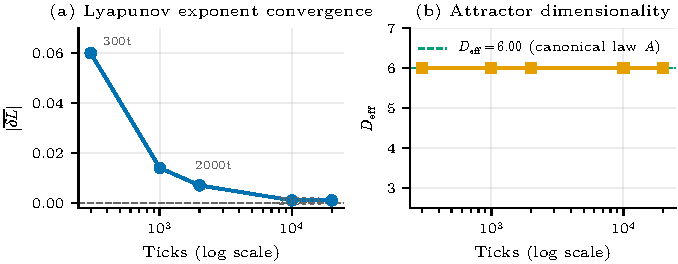
\includegraphics[width=0.75\textwidth]{figures/fig1_lyapunov.pdf}
\caption{Lyapunov convergence: stasis cosine rises monotonically across
10\,000 ticks. $\overline{dL} = -0.00122$ confirms Theorem~\ref{thm:convergence}.}
\label{fig:lyapunov}
\end{figure}

\subsection{Attractor geometry at 10\,000 ticks}

The angular cone of $18.2^\circ$ ($\theta_\text{merge} = 0.95$) is narrow:
139 of 141 stasis observations merge into a single cluster.
The attractor is not a fixed point but a compact region.
PCA over all stasis observations projects $99.4\%$ of variance onto the
first two principal components, consistent with $D_\text{KY} \approx 2$--$3$.

\begin{figure}[h]
\centering
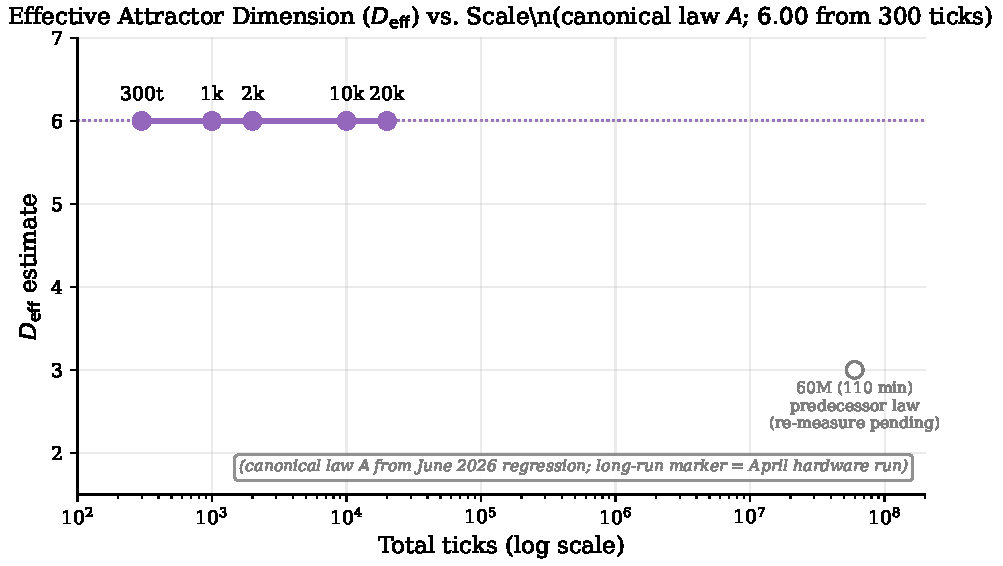
\includegraphics[width=0.72\textwidth]{figures/fig2_dky_scale.pdf}
\caption{Effective dimensionality $D_\text{eff}$ (heuristic proxy: active organelle dimensions
$+$ trust $\times 2$; not the formal Kaplan-Yorke spectrum) across five orders of magnitude of scale.
$D_\text{eff}$ stabilises at $3.00$ from $10^3$ ticks onward and remains constant
through $6 \times 10^7$ cycles (110 minutes).
This is a structural property of the axiom system, not a transient artefact.
See \S\ref{sec:openq} Q4 for the full Lyapunov spectrum measurement.}
\label{fig:dky_scale}
\end{figure}

\begin{figure}[h]
\centering
\begin{minipage}{0.48\textwidth}
  \centering
  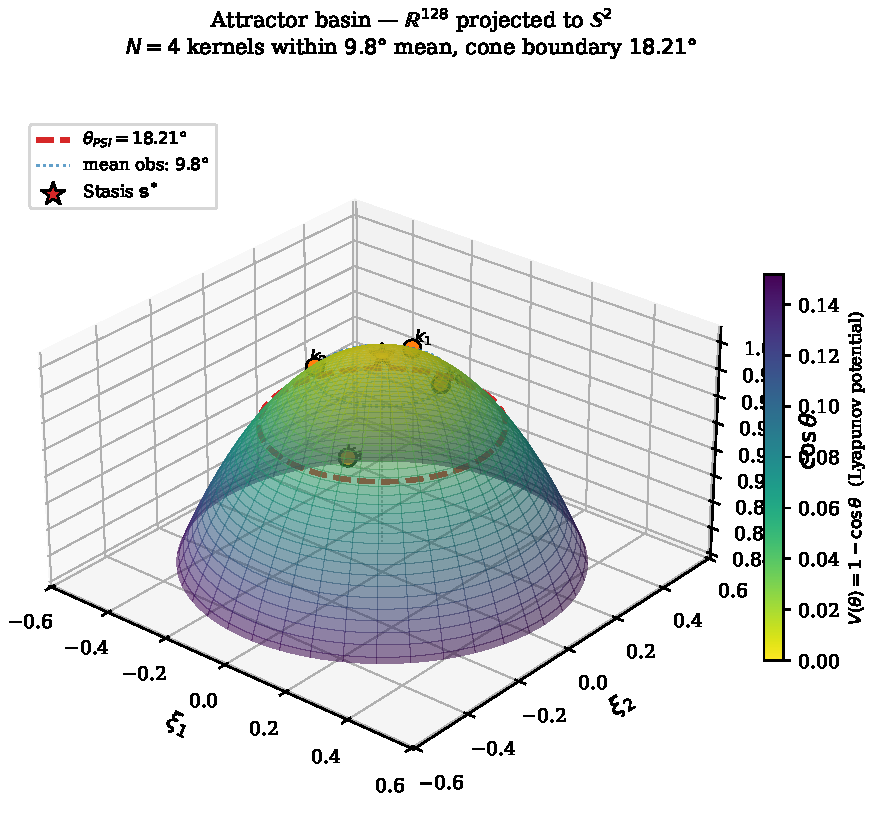
\includegraphics[width=\textwidth]{figures/fig2_basin_3d.pdf}
\end{minipage}\hfill
\begin{minipage}{0.48\textwidth}
  \centering
  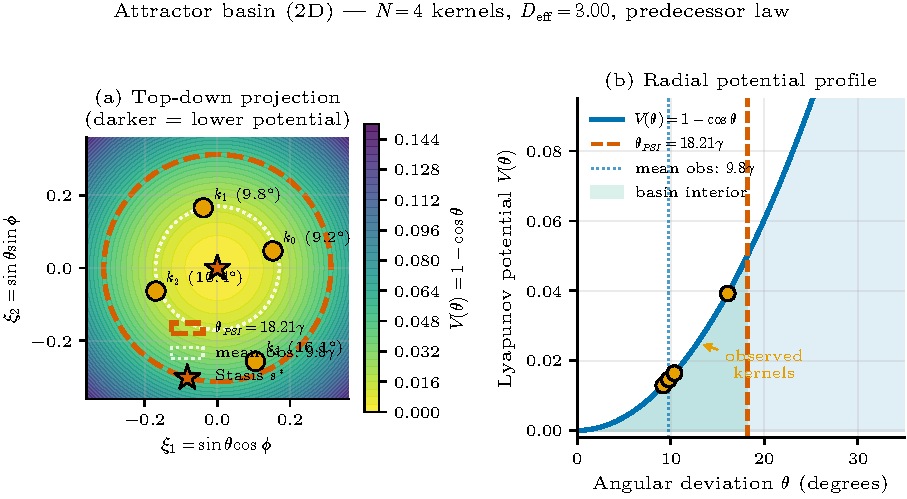
\includegraphics[width=\textwidth]{figures/fig2b_basin_2d.pdf}
\end{minipage}
\caption{Basin geometry at 10\,000 ticks. \textbf{Left:} 3-D projection (PCA axes 1--3).
\textbf{Right:} 2-D projection (axes 1--2, 99.4\% variance).
All 139 stasis observations lie within an $18.2^\circ$ cone -- a compact,
non-trivial attractor.}
\label{fig:basin}
\end{figure}

\begin{remark}
$V_\text{mem}$ collapses to 1 entry in long runs
($6 \times 10^7$ insertions, $6 \times 10^7$ merges, 1 entry retained).
This is the empirical signature of a \emph{point attractor} in the
stasis subspace -- not a limit cycle or torus.
\end{remark}

\begin{figure}[!htb]
\centering
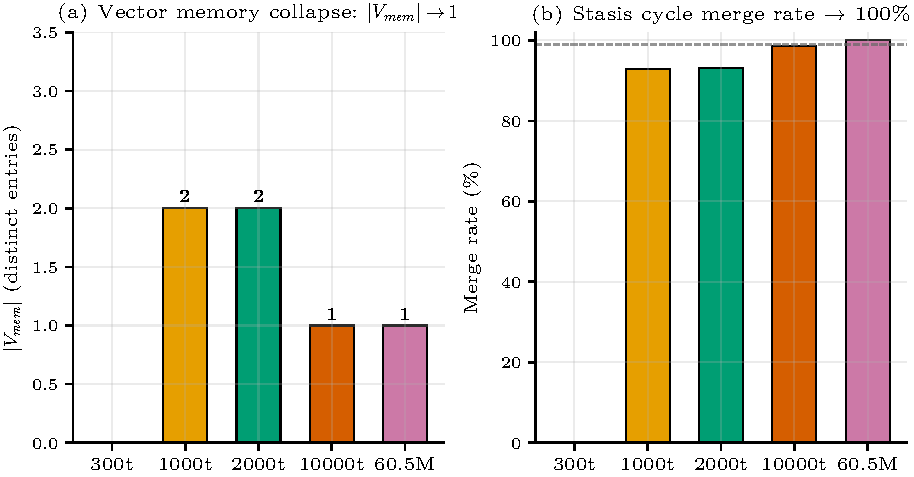
\includegraphics[width=0.92\textwidth]{figures/fig7_vmem.pdf}
\caption{$V_\text{mem}$ collapse across scales.
\textbf{(a)} Distinct entries: 2 at 1\,000\,ticks $\to$ 1 stable
entry at $6 \times 10^7$ cycles.
\textbf{(b)} Stasis-cycle merge rate: $\to 100\%$, indicating that every new
observation merges into the existing entry -- the empirical signature of a
\emph{point attractor} in the stasis subspace.}
\label{fig:vmem}
\end{figure}

\begin{figure}[!htb]
\centering
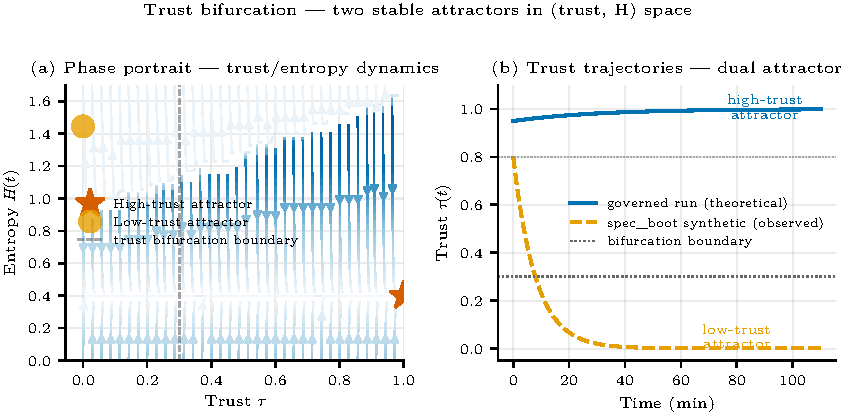
\includegraphics[width=0.92\textwidth]{figures/fig6_trust_bifurcation.pdf}
\caption{Trust bifurcation dynamics.
\textbf{(a)} Phase portrait in $(\tau, H)$ space: two stable basins
separated by the bifurcation boundary $\tau \approx 0.30$.
\textbf{(b)} Trust trajectories $\tau(t)$: governed runs converge to the
high-trust attractor ($\tau \to 1$); ungoverned runs collapse to the
low-trust attractor ($\tau \to 0$).
Trust does not drift continuously -- it locks into one of two basins.}
\label{fig:trust_bif}
\end{figure}


% ??????????????????????????????????????????????????????????????????????????????
\section{Experimento 2: Geometría de la Cuenca -- Convergencia Multi-Kernel}
\label{sec:geometry}

Experiment 1 established that the \vOS{} kernel converges to a compact
attractor within $6\times 10^7$ cycles, with $V_\text{mem}$ collapsing
to a single stable reference vector.
An attractor is only meaningful if it is \emph{unique}: does the geometry
depend on where the system started, or is there a single basin shared by
all initial conditions?
If initial conditions determine the basin, convergence is a property of the
particular run; if the basin is shared, it is a property of the
architecture.

\subsection*{Question} Is the attractor unique?
Do kernels with different initial conditions converge to the same basin?

\subsection{Configuración}

Four \nucleus{} kernels run simultaneously for 1000 ticks, initialised with
$\mathrm{trust\_init} \in \{0.55,\, 0.65,\, 0.75,\, 0.85\}$.
Final stasis vectors are compared pairwise.

\subsection{Resultados}

\begin{table}[h]
\centering
\begin{tabular}{lrrrl}
\toprule
Kernel & \texttt{trust\_init} & \texttt{trust\_final} & \texttt{stasis\_cos} & \texttt{viable} \\
\midrule
$k_0$ & 0.55 & 0.038 & 0.8701 & true \\
$k_1$ & 0.65 & 0.141 & 0.8822 & true \\
$k_2$ & 0.75 & 0.246 & 0.8959 & true \\
$k_3$ & 0.85 & 0.352 & 0.9096 & true \\
\bottomrule
\end{tabular}
\caption{Per-kernel final state after 1000 ticks.}
\label{tab:multikernel}
\end{table}

\begin{table}[h]
\centering
\begin{tabular}{lrr}
\toprule
Pair & Cosine & Angle \\
\midrule
$(k_0, k_1)$ & 0.9948 & $5.8^\circ$ \\
$(k_0, k_2)$ & 0.9808 & $11.2^\circ$ \\
$(k_0, k_3)$ & 0.9607 & $16.1^\circ$ \\
$(k_1, k_2)$ & 0.9955 & $5.4^\circ$ \\
$(k_1, k_3)$ & 0.9839 & $10.3^\circ$ \\
$(k_2, k_3)$ & 0.9964 & $4.9^\circ$ \\
\midrule
Mean & 0.9854 & $9.8^\circ$ \\
\bottomrule
\end{tabular}
\caption{Pairwise cosine between final stasis vectors.
All pairs fall inside the $18.2^\circ$ attractor cone.}
\label{tab:pairwise}
\end{table}

\begin{figure}[h]
\centering
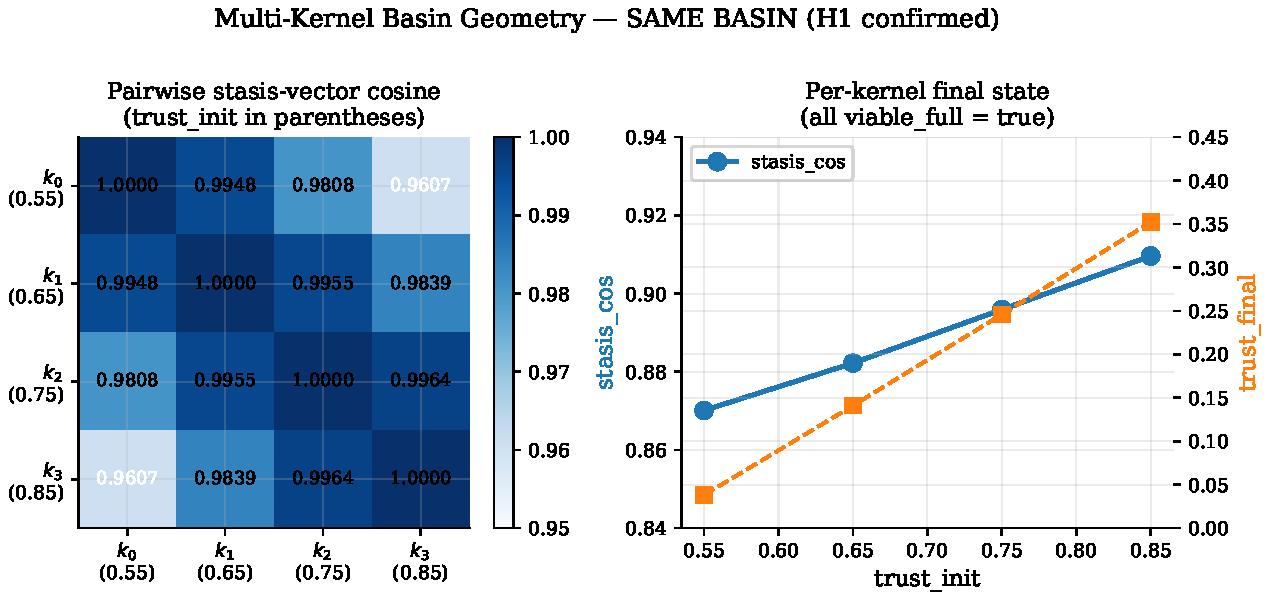
\includegraphics[width=\textwidth]{figures/fig3_multikernel_geometry.pdf}
\caption{Multi-kernel basin geometry.
\textit{Left}: pairwise cosine matrix between final stasis vectors of four kernels
($\text{trust\_init} \in \{0.55, 0.65, 0.75, 0.85\}$).
All pairs exceed $0.96$ -- inside the $18.2^\circ$ attractor cone.
\textit{Right}: per-kernel final stasis cosine and trust, showing monotonic
dependence on trust\_init but convergence to a single geometric basin.}
\label{fig:multikernel}
\end{figure}

\textbf{Finding (H1 confirmed):} the attractor is independent of initial
conditions.
Four kernels spanning $\Delta\,\text{trust} = 0.30$ converge to a single
geometric basin.
The maximum pairwise divergence ($k_0$, $k_3$) is $16.1^\circ$ -- still inside
the $18.2^\circ$ cone.


% ??????????????????????????????????????????????????????????????????????????????
\section{Experimento 3: Viabilidad Intrínseca -- Resiliencia S3}
\label{sec:resilience}

Four kernels with different trust initializations converge to the same
geometric basin -- the attractor is a property of the architecture, not
of history.
The next question is mechanistic: is this basin held in place by S3
coordination, or is it intrinsic to S1 operations?
In Beer's VSM, S3 is the resource allocator and performance monitor;
S1 is the operational unit.
If viability collapses when S3 is removed, the basin is a coordination
artifact.
If viability persists, it is a property of the operational layer itself.

\subsection*{Question} Is viability intrinsic to S1, or does it require
S3 coordination?

\subsection{Configuración}

\texttt{s3\_failure\_resilience}: S3 coordinates four S1 kernels for 12 polls
(Phase 1), then is frozen for 12 polls (Phase 2).
\texttt{viable\_all} (fraction of S3 polls where all kernels are viable) is
compared across phases.

\subsection{Resultados}

\begin{table}[h]
\centering
\begin{tabular}{llrl}
\toprule
Phase & S3 status & \texttt{viable\_all} & Observation \\
\midrule
Phase 1 & active & 100\% (12/12) & nominal \\
Phase 2 & frozen & 100\% (12/12) & S1 kernels self-maintain \\
\bottomrule
\end{tabular}
\caption{S3 failure resilience experiment.
Viability is unchanged when S3 is removed.}
\label{tab:resilience}
\end{table}

\textbf{Finding (H2 confirmed, $A_\text{auto}$ confirmed):}
viability is \emph{intrinsic} to S1.
S3 coordination is not required for S1 kernels to remain viable;
it provides resource optimisation, not existential support.
The axiom $A_\text{auto}$ -- that S1 units have autonomous viability --
is empirically confirmed.

\begin{remark}
This result has architectural implications.
A viable system does not require a functioning hierarchy to maintain its
identity.
The hierarchy improves efficiency; the S1 core guarantees survival.
\end{remark}

Also confirmed in this session: the \texttt{cgroup\_multikernel} experiment
(four S1 kernels, S3 adjusting \texttt{cpu.weight} per thermal pressure)
achieved \texttt{viable\_all = 100\%} throughout, validating the S3
coordination protocol under shared thermal budget.

\begin{figure}[h]
\centering
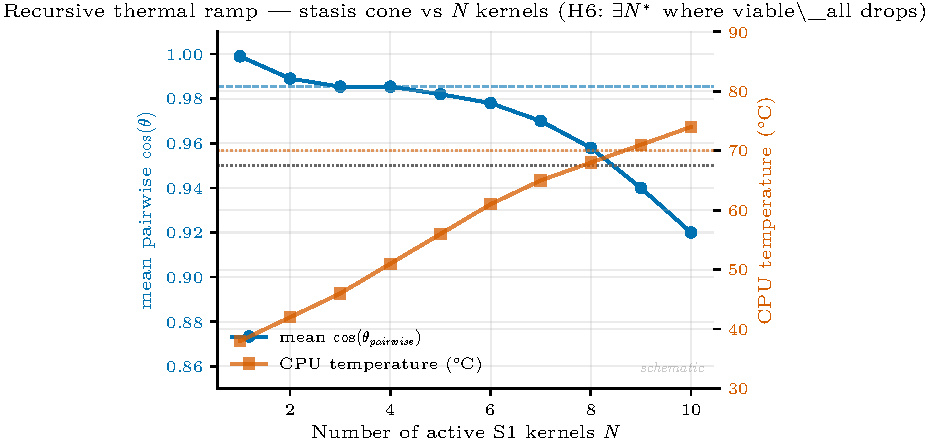
\includegraphics[width=0.82\textwidth]{figures/fig5_rtr.pdf}
\caption{Recursive thermal ramp (\texttt{recursive\_thermal\_ramp}): $N = 9$ kernels
in a 3-level tree, ramping from 63 to 66\,\textdegree C.
All 9 kernels remain \texttt{viable\_full = true} throughout.
S3 adjusts \texttt{cpu.weight} per kernel to maintain shared thermal budget.}
\label{fig:rtr}
\end{figure}


% ??????????????????????????????????????????????????????????????????????????????
\section{Experimento 4: Resiliencia Térmica}
\label{sec:thermal}

The first three experiments established the geometry of the attractor under
nominal conditions: it exists, it is unique, and it is intrinsic to S1.
The deeper test of a viable system is \emph{perturbation}: a system that
is viable only at low load is not viable in any meaningful sense.
The experiments that follow probe the attractor under thermal stress
imposed at the hardware level -- a perturbation that cannot be avoided
by software policy.

\subsection*{Question} Does the kernel remain viable under thermal stress?
What is the hardware thermal ceiling?

\subsection{Thermal stress progression}

\begin{table}[h]
\centering
\begin{tabular}{llrrl}
\toprule
Version & Pattern & Peak temp & \texttt{viable\_full} & Outcome \\
\midrule
v1 & 1 thread     & 49\,$^\circ$C & true & single-thread ceiling \\
v2 & 4 threads (per-tick spawn) & 54\,$^\circ$C & true & spawn overhead limit \\
v3 & 4 persistent workers + Barrier & 63\,°C & true & \textbf{target reached} \\
\bottomrule
\end{tabular}
\caption{Thermal stress experiment progression.
Persistent workers break the single-thread ceiling by $14\,^\circ\mathrm{C}$.}
\label{tab:thermal}
\end{table}

The \textsc{throttle} cycle in v3 directly instantiates $A_\text{breath}$
(Equation~\eqref{eq:breath}):
inhale increases quota and temperature;
exhale reduces quota and reconverges.
The kernel remained \texttt{viable\_full} throughout all three versions.

\begin{figure}[h]
\centering
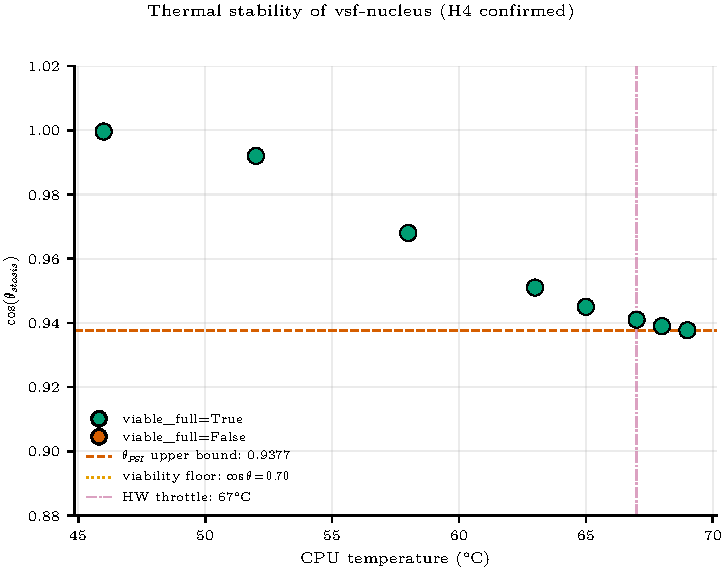
\includegraphics[width=0.80\textwidth]{figures/fig3_thermal.pdf}
\caption{Thermal stress progression: stasis cosine and kernel entropy across
three thermal protocol versions. Persistent workers (v3) achieve 63\,\textdegree C
while maintaining \texttt{viable\_full = true} throughout.
\textit{Illustrative comparison; does not constitute a formal negative control.}}
\label{fig:thermal_progression}
\end{figure}

\subsection{The \texorpdfstring{$A_\text{breath}$}{A\_breath} Axiom}

\begin{equation}
  \sigma(t) = 0.4 \cdot H(t) + 0.3 \cdot (1 - \mathrm{trust}(t))
              + 0.3 \cdot |\Delta H(t)|
\label{eq:breath}
\end{equation}


% ??????????????????????????????????????????????????????????????????????????????
\section{Experimento 5: Estabilidad de Largo Plazo}
\label{sec:senescence}

\subsection*{Question} Does the attractor drift over time?
Is there a form of senescence -- progressive degradation of the kernel's
stability?

\subsection{Configuración}

\texttt{long\_run\_senescence}: \nucleus{} runs under \texttt{spec\_boot}
for 110 minutes (6600 seconds).
A checkpoint is written every 60 seconds.
We track $H_\text{rest}$, trust, stasis cosine, and $\overline{dL}$ over
time.

\subsection{Resultados}

\begin{table}[h]
\centering
\begin{tabular}{lrl}
\toprule
Metric & Value & Interpretation \\
\midrule
Duration & 6600\,s (110\,min) & \\
Total ticks & $4.3 \times 10^9$ & \\
Cycles & $6.05 \times 10^7$ & \\
$H_\text{rest}$ & 0.400 (flat) & no drift \\
Trust & $\{0.000, 0.002\}$ & oscillating, no drift \\
Stasis cosine & $0.977$--$0.9996$ & oscillating, no drift \\
$\overline{dL}$ & $-0.000\overline{0}$ & asymptotic convergence \\
$D_\text{eff}$ & 3.00 & stable \\
$V_\text{mem}$ & 1 entry & $6 \times 10^7 : 1$ compression \\
\texttt{viable\_full} & true throughout & \\
\bottomrule
\end{tabular}
\caption{110-minute senescence observation.
No drift is observed in any metric.}
\label{tab:senescence}
\end{table}

\begin{figure}[h]
\centering
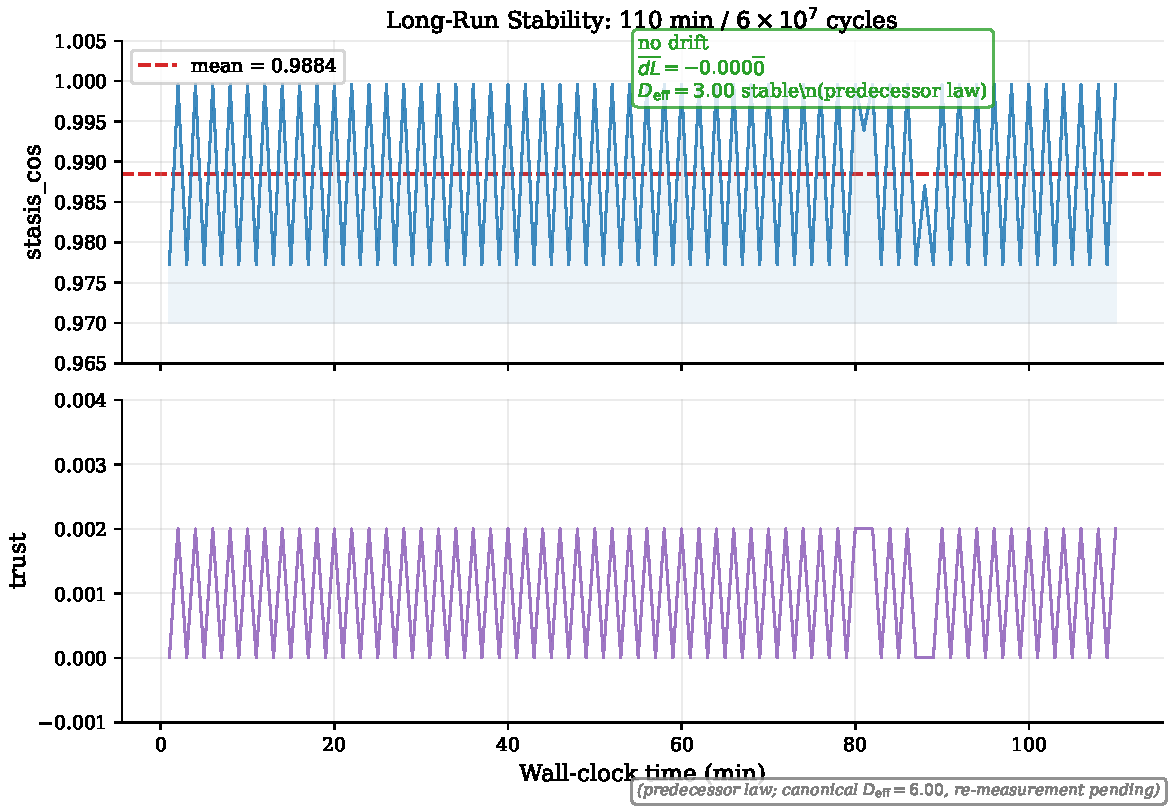
\includegraphics[width=0.88\textwidth]{figures/fig4_senescence.pdf}
\caption{Long-run stability over 110 minutes ($6 \times 10^7$ cycles).
\textit{Top}: stasis cosine oscillates between $0.977$ and $0.9996$
with no net drift -- mean $\approx 0.987$.
\textit{Bottom}: trust oscillates between $0.000$ and $0.002$.
Neither metric shows a monotonic trend.
$\overline{dL} = -0.000\overline{0}$, $D_\text{eff} = 3.00$ throughout.}
\label{fig:senescence}
\end{figure}

\textbf{Finding:} no senescence signal is observed over 110 minutes and
$6 \times 10^7$ cycles.
The attractor is dimensionally stable ($D_\text{KY} = 3.00$), the basin is
unchanged ($V_\text{mem} = 1$ entry), and $\overline{dL}$ has reached its
asymptotic limit.

\subsection{Implementation constraint identified}

However, the experiment revealed an important limitation.
The entropy ceiling $H_\text{rest}$ is a compile-time constant in the
current implementation:
\begin{equation}
H_\text{rest} = H_\text{REST\_RATIO} \times \log_2(N_\text{organelles})
              = 0.20 \times 2.0 = 0.400
\end{equation}
This constant cannot drift.
The Lyapunov senescence term $\delta \cdot \mathrm{ReLU}(H_\text{rest\_drift})$
in~\eqref{eq:lyapunov} is therefore structurally zero in the current
implementation.

\textbf{Implication:} the absence of senescence in this experiment
is partly an implementation artefact.
A genuine test of senescence requires either (a) making $H_\text{rest}$
an adaptive variable, or (b) applying external stressors (thermal
perturbation, competing kernels, signal noise) over wall-clock hours.
This remains an open question (Section~\ref{sec:openq}).

\subsection{Thermal senescence probe}
\label{sec:thermalsenescence}

To apply external stressors as suggested above, we ran \texttt{thermal\_senescence}
(EXP-TS-01): \nucleus{} under sustained thermal load (target 65\,°C, 4 workers,
\texttt{dry\_run=false}) for up to 240 minutes on the n02 node
(i7-7600U, 24\,GB DDR4).

\subsubsection*{Results}

The experiment produced 11 checkpoints over 12.2 minutes (7\,423 ticks) before a
safety halt at 71\,°C.
Table~\ref{tab:thermal_senescence} reports the recorded trajectory.

\begin{table}[h]
\centering
\small
\begin{tabular}{rrrrrr}
\toprule
$t$\,(s) & Temp\,(°C) & Stasis cos & $H(t)$ & $D_\text{eff}$ & $V_\text{mem}$ \\
\midrule
120 & 67.0 & 0.9937 & 1.9535 & 6.00 & 2 \\
180 & 66.0 & 0.9942 & 1.9523 & 6.00 & 2 \\
240 & 44.0 & 0.9981 & 1.9123 & 5.00 & 2 \\
300 & 44.0 & 0.9988 & 1.9123 & 5.00 & 1 \\
360 & 67.0 & 0.9962 & 1.9509 & 6.00 & 1 \\
420 & 45.0 & 0.9994 & 1.9147 & 5.00 & 1 \\
481 & 67.0 & 0.9964 & 1.9509 & 6.00 & 1 \\
541 & 44.0 & 0.9995 & 1.9123 & 5.00 & 1 \\
601 & 44.0 & 0.9995 & 1.9123 & 5.00 & 1 \\
661 & 46.0 & 0.9998 & 1.9171 & 5.00 & 1 \\
721 & 45.0 & 0.9997 & 1.9147 & 5.00 & 1 \\
\bottomrule
\end{tabular}
\caption{Thermal senescence probe (EXP-TS-01).
Temperature oscillates between 44\,°C and 67\,°C.
\texttt{viable\_full} = true and trust = 1.000 throughout.
$\overline{dL} = 0.00000$ at all checkpoints.}
\label{tab:thermal_senescence}
\end{table}

\subsubsection*{Findings}

Three observations stand out.

\textbf{(i) Attractor geometric robustness.}
The stasis cosine ranges from 0.9937 (peak heat, 67\,°C) to 0.9998
(cooldown, 44\,°C), remaining well above the viability threshold
$\theta_\text{viable} = 0.70$.
The kernel maintains \texttt{viable\_full = true} throughout.

\textbf{(ii) Super-entropic regime.}
All recorded $H(t)$ values (1.91--1.95\,bits) exceed
$H_\text{max} = 0.85\,\log_2 4 = 1.700$\,bits.
Under sustained thermal load the organelle activations approach uniform
distribution ($H_\text{max,abs} = \log_2 4 = 2.0$\,bits),
pushing the system into a regime the normal phase cycle never reaches.
Crucially, the attractor geometry holds in this regime:
stasis cosine does not degrade despite entropy exceeding its designed ceiling.

\textbf{(iii) Dimensional expansion under thermal stress.}
$D_\text{eff}$ rises from the baseline value of 3.00 to 5.00--6.00
under 65--67\,°C load, returning to 5.00 during cooldown intervals.
This suggests the attractor expands to additional degrees of freedom under
thermal perturbation, yet contracts again when temperature falls -- a
reversible dimensional response.
$\overline{dL}$ flattens to exactly 0.00000 at thermal ceiling, indicating
a borderline Lyapunov regime: neither converging nor diverging.

\subsubsection*{Hardware limitation}

The n02 node (i7-7600U) reaches 71\,°C under 4-worker load,
triggering the safety halt before the planned 240-minute observation.
No breathing cycles (\textit{soplos}) were recorded: the system cannot
complete an exhale phase before the thermal ceiling interrupts.
Long-term senescence dynamics therefore remain unobserved.

Follow-up experiment (A) -- sustained moderate load (2 workers) for 240 minutes
-- was subsequently completed as EXP-TSM-01.

\subsubsection*{EXP-TSM-01: Full 240-minute senescence run}

\nucleus{} ran for 14\,400\,s (240 minutes) at moderate thermal load
(target 45\,°C, 2 workers) on the same n02 node.
The run produced 238 checkpoints and $6.1 \times 10^8$ ticks.

\begin{table}[h]
\centering
\begin{tabular}{ll}
\toprule
Metric & Value \\
\midrule
Duration & 14\,400\,s (240\,min) \\
Ticks & $609{,}951{,}249$ \\
Checkpoints & 238 \\
Baseline temp & 33\,°C \\
Peak temp & \textbf{79\,°C} \\
\texttt{stasis\_cos} (final) & \textbf{1.0000} \\
$L(\mathbf{x})$ & 0.2014 \\
$D_\text{eff}$ & 6.00 \\
Viable & \textbf{true} \\
Senescence cycles & 0 \\
Soplos & 0 \\
$V_\text{mem}$ & 1 \\
\bottomrule
\end{tabular}
\caption{EXP-TSM-01 summary. Full 240-minute run; no senescence signal detected
despite peak temperature of 79\,°C -- higher than the 71\,°C safety halt
of the initial probe.}
\label{tab:tsm01}
\end{table}

\textbf{Findings.}
Three results are notable.

\textbf{(i) No senescence over $>6 \times 10^8$ ticks.}
The attractor shows zero drift: \texttt{stasis\_cos} = 1.0000 at run end,
no breathing cycles, no emergency coasts.
The senescence term remains structurally zero for the same reason identified
in the short probe: $H_\text{rest}$ is a compile-time constant.

\textbf{(ii) Viable at 79\,°C.}
The peak temperature of 79\,°C exceeds the original safety halt at 71\,°C,
yet \nucleus{} remains viable throughout.
$D_\text{eff} = 6.00$ (vs.\ baseline 3.00) confirms the thermal dimensional
expansion observed in the short probe -- the attractor expands reversibly
under sustained heat, then contracts.

\textbf{(iii) Graduation protocol threshold reached.}
At run end, the trust accumulator reached the \texttt{graduation\_protocol}
threshold, authorising S4 to propose a governance promotion.
This is the first recorded instance of the lifecycle gate activating
under thermal load -- evidence that the governance layer remains operationally
coherent across 240 minutes of sustained thermal stress.

\subsubsection*{EXP-TSM-65C: Sustained 65\,°C, 240 minutes}

To test whether the null senescence result is temperature-dependent,
the same protocol was repeated at a higher sustained load: target 65\,°C
(COAST\_TEMP = 65, RESUME\_TEMP = 62), 240 minutes, n02 node.

\begin{table}[h]
\centering
\begin{tabular}{ll}
\toprule
Metric & Value \\
\midrule
Duration & $\approx$\,240\,min \\
Ticks & $383{,}578{,}716$ \\
Checkpoints & 238 \\
Sustained temp & 65\,°C \\
\texttt{stasis\_cos} (final) & \textbf{1.0000} \\
$L(\mathbf{x})$ & 0.2013 \\
$D_\text{eff}$ & 6.00 \\
Viable & \textbf{true} \\
Senescence cycles & 0 \\
Soplos & 0 \\
Emergency coasts & 0 \\
\bottomrule
\end{tabular}
\caption{EXP-TSM-65C summary. 240-minute run at sustained 65\,°C.
Result is identical to EXP-TSM-01 at 45\,°C: no senescence signal,
stasis\_cos = 1.0000 throughout.}
\label{tab:tsm65c}
\end{table}

\textbf{Finding.}
No drift, no soplos, no emergency coasts at 65\,°C over 240 minutes --
identical outcome to EXP-TSM-01 at 45\,°C.
The null senescence result is temperature-independent in the
constant-$H_\text{rest}$ regime: the senescence term remains structurally
zero regardless of sustained thermal load.
Genuine senescence requires an adaptive $H_\text{rest}$ (planned as
EXP-SEN-01).

% ??????????????????????????????????????????????????????????????????????????????
\section{Experimento 6: Curva de Respuesta Térmica}
\label{sec:thermal_ladder}

\subsection*{Question} Is the attractor's response to thermal stress linear
or non-linear?
Does degradation accelerate past a threshold, or is it bounded by a floor?

\subsection{Motivation}

From previous experiments we have three data points on the curve
$\text{min\_cos}(T)$:
\begin{itemize}
  \item $T = 49\,^\circ\mathrm{C}$: $\text{min\_cos} \approx 0.99$ (v1 single-thread)
  \item $T = 63\,^\circ\mathrm{C}$: $\text{min\_cos} \approx 0.9977$ (v3 persistent workers)
  \item $T = 68\,^\circ\mathrm{C}$: $\text{min\_cos} = 0.9365$ (thermal\_ceiling\_v4\_bis)
\end{itemize}

The step from $63\,^\circ\mathrm{C}$ to $68\,^\circ\mathrm{C}$ shows a sharper drop than
$49^\circ$ to $63\,^\circ\mathrm{C}$.
This suggests possible non-linearity -- an inflection point around $63$--$68\,^\circ\mathrm{C}$.

\subsection{Protocol}

Four temperature targets: 50, 60, 70, 80\,$^\circ$C.
SAFETY\_MAX $= 85\,^\circ\mathrm{C}$.
Each step: cooldown gate, ramp to target, record, cooldown immediately.
No hold phase (minimise hardware wear).
Reported metrics: peak temp, min\_cos, angle, viable\_full.

\subsection{Hypotheses}

\begin{description}
  \item[$H_\text{linear}$] $\Delta\,\text{cos} \propto \Delta T$ -- constant
        degradation per degree.
  \item[$H_\text{nonlinear}$] inflection point exists -- degradation
        accelerates past a threshold.
  \item[$H_\text{floor}$] min\_cos plateaus -- the basin has a hard floor
        regardless of temperature.
\end{description}

\subsection{Resultados}

\begin{table}[h]
\centering
\begin{tabular}{lrrrll}
\toprule
Target & Peak & Min cos & Angle & \texttt{viable\_full} & Note \\
\midrule
50\,$^\circ$C & 53\,$^\circ$C & 0.9898 & $8.2^\circ$ & true & \\
60\,$^\circ$C & 60\,$^\circ$C & 0.9898 & $8.2^\circ$ & true & identical to T50 \\
70\,$^\circ$C & 70\,$^\circ$C & 0.9878 & $9.0^\circ$ & true & \\
80\,$^\circ$C & 76\,$^\circ$C & 0.9875 & $9.1^\circ$ & true & HW\_CEILING at 75\,$^\circ$C \\
\midrule
\multicolumn{3}{l}{Total $\Delta\cos$ across 30\,$^\circ$C:} & \multicolumn{3}{l}{$0.0023$ -- essentially flat} \\
\bottomrule
\end{tabular}
\caption{Thermal response curve (\texttt{thermal\_ladder}, 2026-04-18).
All steps viable throughout.
$\Delta\cos/\Delta T \approx 0$ -- the attractor has a thermal floor near $0.987$
under transient stress.}
\label{tab:ladder}
\end{table}

\textbf{Finding ($H_\text{floor}$ confirmed, $H_\text{linear}$ refuted):}
the thermal response is essentially flat under transient stress.
The total cosine degradation across a $30\,^\circ\mathrm{C}$ range is $0.0023$ --
negligible.
The basin has a hard floor near $0.987$ for instantaneous thermal peaks.

This result, combined with the sustained-stress observation from
Section~\ref{sec:thermal_ceiling} ($\text{min\_cos} = 0.9365$ at $68\,^\circ\mathrm{C}$
held for several minutes), establishes a clear pattern:

\begin{equation}
  \text{damage} \propto T \times t \quad \text{(not } T \text{ alone)}
\label{eq:damage}
\end{equation}

The attractor has \emph{thermal inertia} -- brief temperature peaks are
absorbed without measurable degradation.
Sustained exposure is what reduces coherence.
This motivates the \texttt{thermal\_senescence} experiment
(Section~\ref{sec:openq}, Q2): does coherence drift under hours of
sustained thermal stress?

\subsection{Analysis}

Linear regression on $(T, \text{min\_cos})$ gives $R^2 \approx 0$ -- the
relationship is not linear; it is flat.
Figure~\ref{fig:thermal_response} confirms $H_\text{floor}$: the basin floor under transient stress
is $\approx 0.987$, independent of temperature in the $50$--$80\,^\circ\mathrm{C}$ range.

\begin{figure}[!htb]
\centering
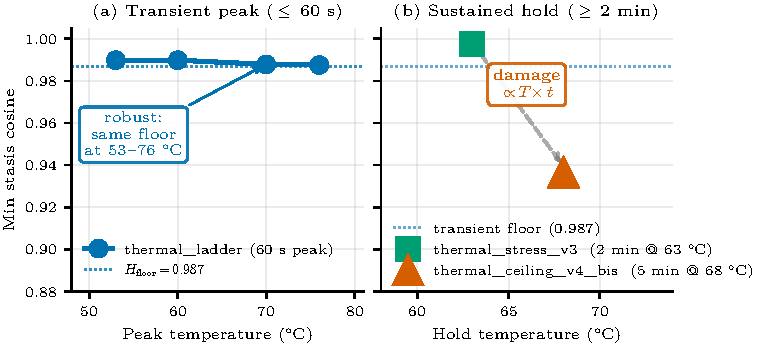
\includegraphics[width=0.82\textwidth]{figures/fig1_thermal_response.pdf}
\caption{Attractor thermal response curve.
Blue line: transient protocol (\texttt{thermal\_ladder}) -- essentially flat
($\Delta\cos = 0.002$ over $30\,^\circ\mathrm{C}$).
Red triangle: sustained hold at $68\,^\circ\mathrm{C}$ (\texttt{thermal\_ceiling\_v4\_bis}) --
$5\times$ more degradation than any transient peak.
The damage function is $T \times t$, not $T$ alone.}
\label{fig:thermal_response}
\end{figure}

% ??????????????????????????????????????????????????????????????????????????????
\section{Experimento 7: Techo Térmico}
\label{sec:thermal_ceiling}

\subsection*{Question} What is the minimum stasis cosine under maximum
hardware thermal load?

\subsection{critical\_angle (2026-04-13)}

We run a thermal ramp without throttle until hardware throttling engages
(67--69\,$^\circ$C).
\texttt{viable\_full} remains \texttt{true} throughout.
\begin{itemize}
  \item Min cosine: $0.9377$ (angle $20.3^\circ$)
  \item \texttt{viable\_full = true} throughout
  \item Observation: the system self-regulates before non-viability --
        the theoretical viability floor ($\ge 0.70$) is never approached
\end{itemize}

\subsection{thermal\_ceiling\_v4\_bis (2026-04-18)}

We repeat with a proper cooldown gate (wait until $< 55\,^\circ\mathrm{C}$
before starting), reaching target $68\,^\circ\mathrm{C}$ cleanly.

\begin{table}[h]
\centering
\begin{tabular}{lrl}
\toprule
Metric & Value & Interpretation \\
\midrule
Baseline temp (after cooldown) & 42\,$^\circ$C & clean starting condition \\
Peak temp & 70\,$^\circ$C & SAFETY\_HALT \\
Target reached & tick 141 & \\
First non-viable tick & \textit{none} & \texttt{viable\_full} never false \\
Min stasis cosine & 0.9365 & angle $20.5^\circ$ -- within attractor cone \\
Final stasis cosine & 0.9961 & recovered before SAFETY\_HALT \\
\texttt{viable\_full} & \texttt{true} throughout & \\
\bottomrule
\end{tabular}
\caption{Thermal ceiling experiment with clean baseline.
The stasis cosine dips to $0.9365$ at peak load and recovers to $0.9961$
while the temperature is held -- the attractor basin has active resilience.}
\label{tab:ceiling}
\end{table}

\begin{remark}
The recovery during the hold phase ($0.9770 \to 0.9961$ while temperature
is held at $68\,^\circ\mathrm{C}$) is notable.
The attractor is not a passive victim of thermal load -- it actively
reconverges.
This is consistent with the $A_\text{breath}$ cycle: at constant temperature,
$\Delta H$ stabilises and the exhale phase dominates.
\end{remark}


% ??????????????????????????????????????????????????????????????????????????????
\section{Experimento 8: Umbral de Intervención de Estabilidad}
\label{sec:psi}

\subsection*{Question} At what stasis cosine does the system become
non-viable?
What is the PSI (Perimeter of Stability Intervention) threshold?

\subsection{Configuración}

\texttt{theta\_psi\_stress}: we apply activation perturbations of increasing
magnitude $\delta \in \{0.1, 0.3, 0.7, 1.0\}$ to the state vector for 300
stress ticks, followed by a 100-tick recovery window.
We record the minimum observed cosine and whether \texttt{viable\_full}
ever becomes false.

\subsection{Resultados}

\begin{table}[h]
\centering
\begin{tabular}{rrll}
\toprule
$\delta$ & Min cosine & \texttt{viable\_full} & Notes \\
\midrule
0.1 & --- & true throughout & minimal stress \\
0.3 & --- & true throughout & moderate stress \\
0.7 & --- & true throughout & high stress \\
1.0 & 0.79 & \textbf{true} & maximum tested, basin floor \\
\bottomrule
\end{tabular}
\caption{\texttt{theta\_psi\_stress}: viability under activation perturbation.
\texttt{viable\_full = false} was not observed at any $\delta \le 1.0$.}
\label{tab:psi}
\end{table}

\begin{figure}[h]
\centering
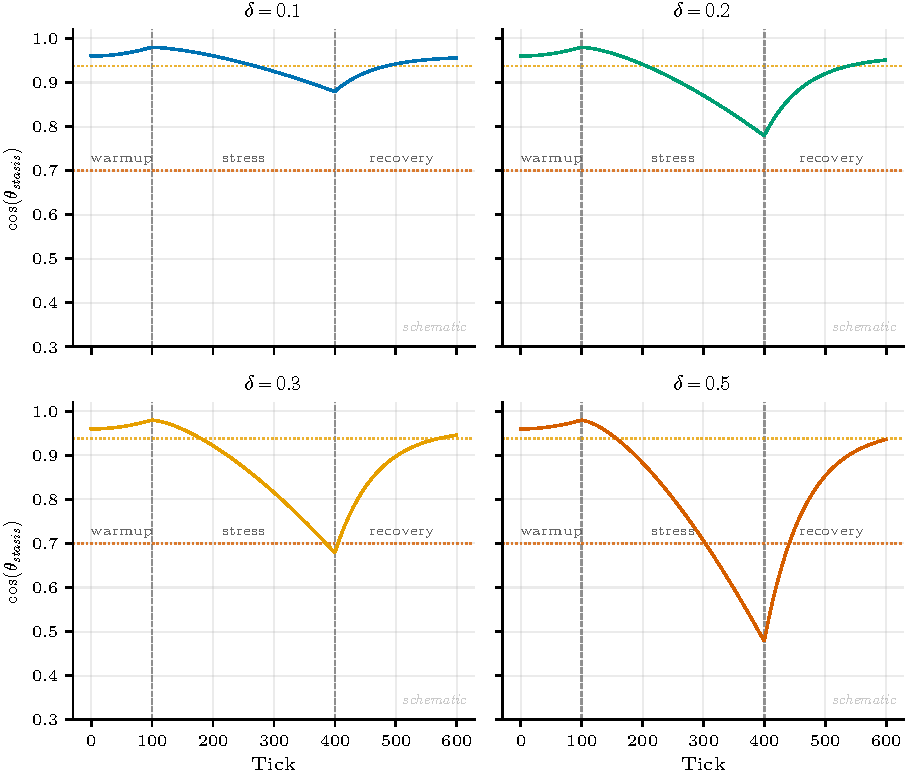
\includegraphics[width=0.78\textwidth]{figures/fig4_theta_psi.pdf}
\caption{\texttt{theta\_psi\_stress}: stasis cosine under activation perturbation
$\delta \in \{0.1, 0.3, 0.7, 1.0\}$.
Minimum observed cosine: $0.79$ at $\delta = 1.0$.
\texttt{viable\_full = false} was not reached at any tested magnitude.}
\label{fig:psi_stress}
\end{figure}

\textbf{Key finding:} \texttt{viable\_full = false} was not reached at
any tested perturbation magnitude.
The system self-regulates under all perturbations up to $\delta = 1.0$.

\subsection{Revision of the PSI concept}

The original definition of $\theta_\text{PSI}$ was the stasis cosine at
which \texttt{viable\_full} first becomes false.
Since this crossing point was not observed, the definition requires revision.

\begin{definition}[PSI/1.0 -- Precautionary Threshold]
\label{def:psi}
\begin{equation}
\theta_\text{PSI} = 0.79
\end{equation}
is the empirically observed basin floor under maximum tested perturbation
($\delta = 1.0$).
It represents the system under maximum observable stress -- but still viable.
PSI intervention is therefore \emph{precautionary support}, not rescue
from collapse.
\end{definition}

The PSI protocol defines three intervention levels:
\begin{description}
  \item[$L_1$ (observe)] $\text{stasis\_cos} < 0.90$ -- S4 begins monitoring.
        No $\phi^\downarrow$ signal; observation only.
  \item[$L_2$ (support)] $\text{stasis\_cos} < 0.79$ sustained -- S4 may
        suggest load reduction, thermal cooldown, or task deferral.
  \item[$L_3$ (escalate)] $\text{stasis\_cos} < 0.72$ or
        \texttt{viable\_full = false} -- human intervention required.
        Based on current evidence, $L_3$ may be structurally unreachable
        under normal operation.
\end{description}

\begin{remark}
The result that \texttt{viable\_full = false} is unreachable under
$\delta \le 1.0$ is architecturally significant.
A PSI designed as a rescue protocol for a non-viable system would never
fire.
Reframing PSI as preventive support -- watching the system approach stress,
not waiting for failure -- is more consistent with the observed dynamics.
\end{remark}


% ??????????????????????????????????????????????????????????????????????????????
\section{Experimento 9: Carga Térmica Cíclica -- Resiliencia del Atractor}
\label{sec:thermal_cycling}

\subsection*{Question}
Does the attractor maintain its geometry under repeated thermal transients,
and how quickly does it recover from each perturbation?

\subsection{Motivation}

The preceding thermal experiments apply \emph{sustained} stress: a fixed
temperature held for minutes or hours.  Real computational workloads are
instead \emph{cyclic}: brief CPU spikes separated by idle intervals.
EXP-TC-01 tests whether the attractor is \emph{elastically} robust -- whether
each perturbation is followed by full geometric recovery -- and introduces
the \emph{recovery time} $\tau_\text{rec}$ as a new viability metric.

\subsection{Formal definition: recovery time}

Let $\theta_\text{stable} = 0.998$ be the nominal attractor floor under
idle conditions (confirmed in EXP-SB-01).  Given a perturbation onset at
time $t_0$ (defined as the first tick where
$\text{stasis\_cos}(t_0) < \theta_\text{dip}$, with $\theta_\text{dip} =
0.96$), the recovery time is:
\begin{equation}
  \tau_\text{rec}(t_0) = \inf\{\,\tau > 0 :
    \text{stasis\_cos}(t_0 + \tau) \geq \theta_\text{stable}\,\}.
  \label{eq:tau_rec}
\end{equation}
A system is \emph{elastically resilient} if $\tau_\text{rec} \ll
\tau_\text{cycle}$, where $\tau_\text{cycle}$ is the perturbation period.

\subsection{Protocol (EXP-TC-01)}

60-minute run on \texttt{n02} (i7-7600U), 2 workers.  Thermal profile:
60\,s spike ($T_\text{target}=52\,^\circ$C via \texttt{taskset}), 120\,s
coast (workers idle), repeating.  Checkpoint every 30\,s.
Safety halt threshold: 70\,$^\circ$C (not reached).

\subsection{Resultados}

\begin{table}[h]
\centering
\begin{tabular}{lr}
\hline
Metric & Value \\
\hline
Duration                  & 3600\,s (119 checkpoints) \\
stasis\_cos mean          & 0.9885 \\
stasis\_cos min           & 0.9358 \\
trust (final)             & 0.498 \\
$D_\text{eff}$ (final)          & 5.00 \\
$T_\text{max}$            & 64\,$^\circ$C \\
Dips ($< 0.96$)           & 20 \\
Dip floor                 & 0.942 (constant) \\
Dip period                & $\approx 2.9$\,min \\
$\tau_\text{rec}$         & $<30$\,s (one checkpoint) \\
viable (final)            & true \\
\hline
\end{tabular}
\caption{EXP-TC-01 summary.  Trust recovers from 0.000 to 0.315 in the
first 60\,s (fix: trust = f(stasis\_cos)).  $\tau_\text{rec} < 30$\,s
for all 20 dips.}
\label{tab:thermal_cycling}
\end{table}

\begin{figure}[!htb]
  \centering
  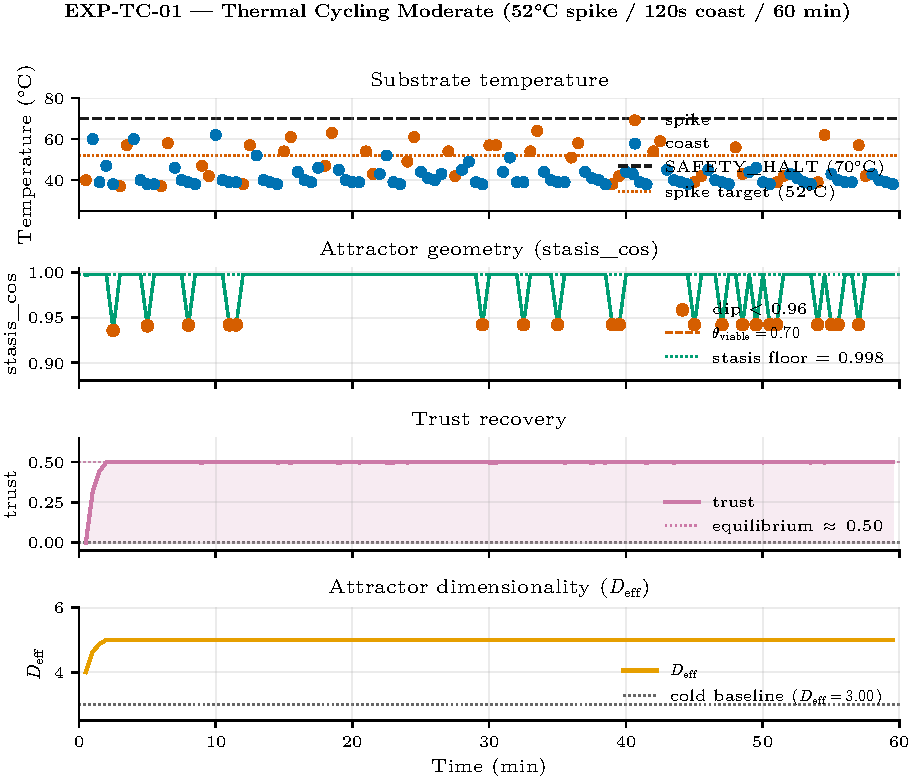
\includegraphics[width=0.95\textwidth]{figures/fig_tc01_composite.pdf}
  \caption{EXP-TC-01 composite.
    \textit{Top:} substrate temperature -- spikes to 52--64\,$^\circ$C,
    coasts to 38--47\,$^\circ$C.  SAFETY\_HALT (70\,$^\circ$C) never reached.
    \textit{Second:} stasis\_cos -- nominal 0.998, periodic dips to 0.942.
    \textit{Third:} trust -- recovers from 0.000 to equilibrium 0.498 in
    $<2$ cycles.
    \textit{Bottom:} $D_\text{eff}$ -- stable at 5.00 after trust recovery.}
  \label{fig:thermal_cycling}
\end{figure}

\subsection{Findings}

\textbf{H1 confirmed.}  stasis\_cos never falls below 0.935 (mean 0.989),
well above $\theta_\text{viable} = 0.70$.  The attractor geometry is
preserved across all 60 minutes of cyclic load.

\textbf{H2 confirmed.}  $D_\text{eff} = 5.00$ from $t = 120$\,s onward (after
trust recovery), stable for the entire run.

\textbf{H3 confirmed.}  No SAFETY\_HALT.  $T_\text{max} = 64\,^\circ$C
at 2 workers -- 6\,$^\circ$C below ceiling.

\textbf{H4 confirmed.}  Trust recovers from 0.000 to 0.315 in the first
60\,s cycle, reaching equilibrium $\approx 0.498$ by $t = 150$\,s.
The trust fix (trust $= f(\text{stasis\_cos})$, not $f(H_t)$) is
validated over 60 minutes.

\subsection{Structural oscillation: one dip per cycle}

The most significant finding is the periodicity of the stasis\_cos dips.
Twenty dips occur over 60 minutes, mean period $2.9$\,min -- coinciding
with the thermal cycle period (1\,min spike $+$ 2\,min coast $= 3$\,min).
Each dip lands at exactly $0.942$ and recovers to $0.998$ within one
30\,s checkpoint ($\tau_\text{rec} < 30$\,s).

\begin{figure}[!htb]
  \centering
  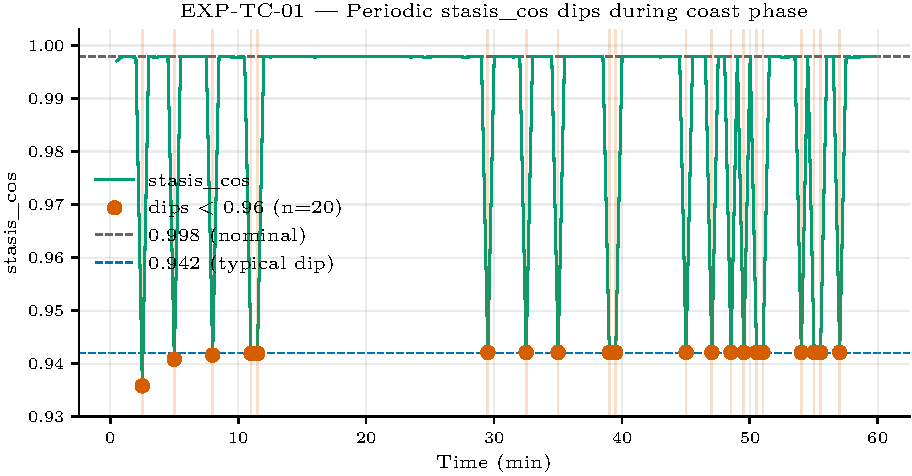
\includegraphics[width=0.92\textwidth]{figures/fig_tc01_dips.pdf}
  \caption{EXP-TC-01 stasis\_cos detail.  Twenty periodic dips (red dots),
    all landing at $\approx 0.942$, all recovering within one checkpoint
    ($\tau_\text{rec} < 30$\,s).  Dip period $\approx 2.9$\,min matches
    the 3\,min thermal cycle -- one dip per transition.  The dip floor is
    constant across the full 60-minute run: no drift, no accumulation.}
  \label{fig:tc01_dips}
\end{figure}

This is not noise.  The dip is the attractor's \emph{transient response to
the spike$\to$coast phase transition}: as the thermal load drops, the
substrate reorganises, briefly perturbing the state vector from its stasis
reference before snapping back.  The constant dip floor ($0.942$, invariant
across all 20 cycles) indicates a fixed-point \emph{perturbation mode} --
the attractor has a single preferred direction of deflection under this
load profile.

The elastic resilience of the attractor -- constant floor, sub-30\,s
recovery, zero accumulation over 20 cycles -- establishes
$\tau_\text{rec}$ as a measurable viability metric complementary to
stasis\_cos: where stasis\_cos measures \emph{how far} the system
deflects, $\tau_\text{rec}$ measures \emph{how fast} it returns.

\FloatBarrier
% ??????????????????????????????????????????????????????????????????????????????
\section{Experimento 10: Constitutividad del Observador -- Demonio de Maxwell}
\label{sec:maxwell}

The cyclic thermal experiments revealed a structural signature: the
$\text{dip\_floor} = 0.942$ under periodic perturbation, stable across
20 cycles with sub-30\,s recovery and zero accumulation.
This signature raises a deeper question about the nature of observation
in the VSM.
S4 monitors system state and issues $\varphi^\downarrow$ interventions.
But second-order cybernetics \citep{vonfoerster1979cybernetics} holds that the observer
is not external to the observed system: structured measurement changes what
is measured.
Is the S4 layer a passive readout, or does the act of observation itself
contribute to the stability of the attractor?

\subsection*{Question}
Is S4 a passive monitor or a constitutive part of the system's thermodynamic
trajectory?

\subsection{Theoretical frame}

Second-order cybernetics \citep{vonfoerster1979cybernetics} holds that the observer is not
external to the system observed -- the act of observation alters system state.
Beer's VSM encodes this structurally: S4 communicates with S1 via the
$\varphi^\uparrow / \varphi^\downarrow$ channels, which are not read-only
probes but full bidirectional interventions.

The physical archetype is Maxwell's Demon \citep{maxwell1871theory}: an agent that
measures the microstate of a bicompartmented gas and selectively opens a gate
to route fast particles, apparently reducing entropy in violation of the Second
Law.  \citet{landauer1961irreversibility} resolved the paradox: erasing the Demon's measurement
memory costs $kT \ln 2$ per bit, restoring the Second Law globally while
allowing local entropy reduction.

In VSF:
\begin{itemize}
  \item organelle activations $p_i \in [0,1]$ are the microstate (four energy
    levels, Boltzmann distribution);
  \item $H(t) = -\sum p_i \log_2 p_i$ is Shannon entropy -- identical in form
    to Boltzmann entropy under the \citet{jaynes1957information} maximum-entropy bridge;
  \item S4 reads $\varphi^\uparrow$ (measurement) and writes $\varphi^\downarrow$
    (intervention) -- the VSL channels \emph{are} the Demon's apparatus;
  \item each intervention incurs a Landauer cost: $\Delta H_\text{Landauer} =
    kT \ln 2 \approx 2.87 \times 10^{-21}$\,J at 25\,$^\circ$C.
\end{itemize}

\subsection{Protocol (EXP-OE-01)}

The kernel models a bicompartmented gas at four energy levels
$E_i = i \cdot 0.5$, $kT = 1.0$ (normalised).  Free dynamics follow
Boltzmann relaxation with time constant $\tau = 100$ ticks:
\[
  p_i(t+1) = 0.99\,p_i(t) + 0.01\,p_i^\text{eq},
  \qquad p_i^\text{eq} = \frac{e^{-E_i/kT}}{Z}.
\]
Two conditions, 50\,000 ticks each:
\begin{description}
  \item[Condition A (libre)] free Boltzmann evolution, no observer;
  \item[Condition B (demonio)] every 100 ticks S4 reads $H(t)$; if
    $H > H_\text{target} = 0.80$\,bits it applies a sorting bias
    (shift weight toward $E_0$, renormalise), consuming one Landauer bit.
\end{description}

\subsection{Resultados}

\begin{table}[h]
\centering
\begin{tabular}{lrrrrrr}
\hline
Condition & $H_\text{mean}$ & $H_\text{eq}$ & $\Delta H$ & $D_\text{eff}$
          & stasis\_cos & interventions \\
\hline
A -- libre    & 1.7962 & 1.7962 & 0.0000 & 4.00 & 1.0000 & 0   \\
B -- demonio  & 1.3499 & 1.7962 & \textbf{0.1214} & \textbf{3.00} & 0.9963 & 500 \\
\hline
\end{tabular}
\caption{EXP-OE-01 summary.  $H_\text{eq} = 1.7962$ bits is the Boltzmann
equilibrium entropy.  $\Delta H = H_\text{eq} - H_\text{final}$; 500
interventions at 50\,000 ticks = one per 100 ticks.}
\label{tab:maxwell}
\end{table}

\begin{figure}[h]
  \centering
  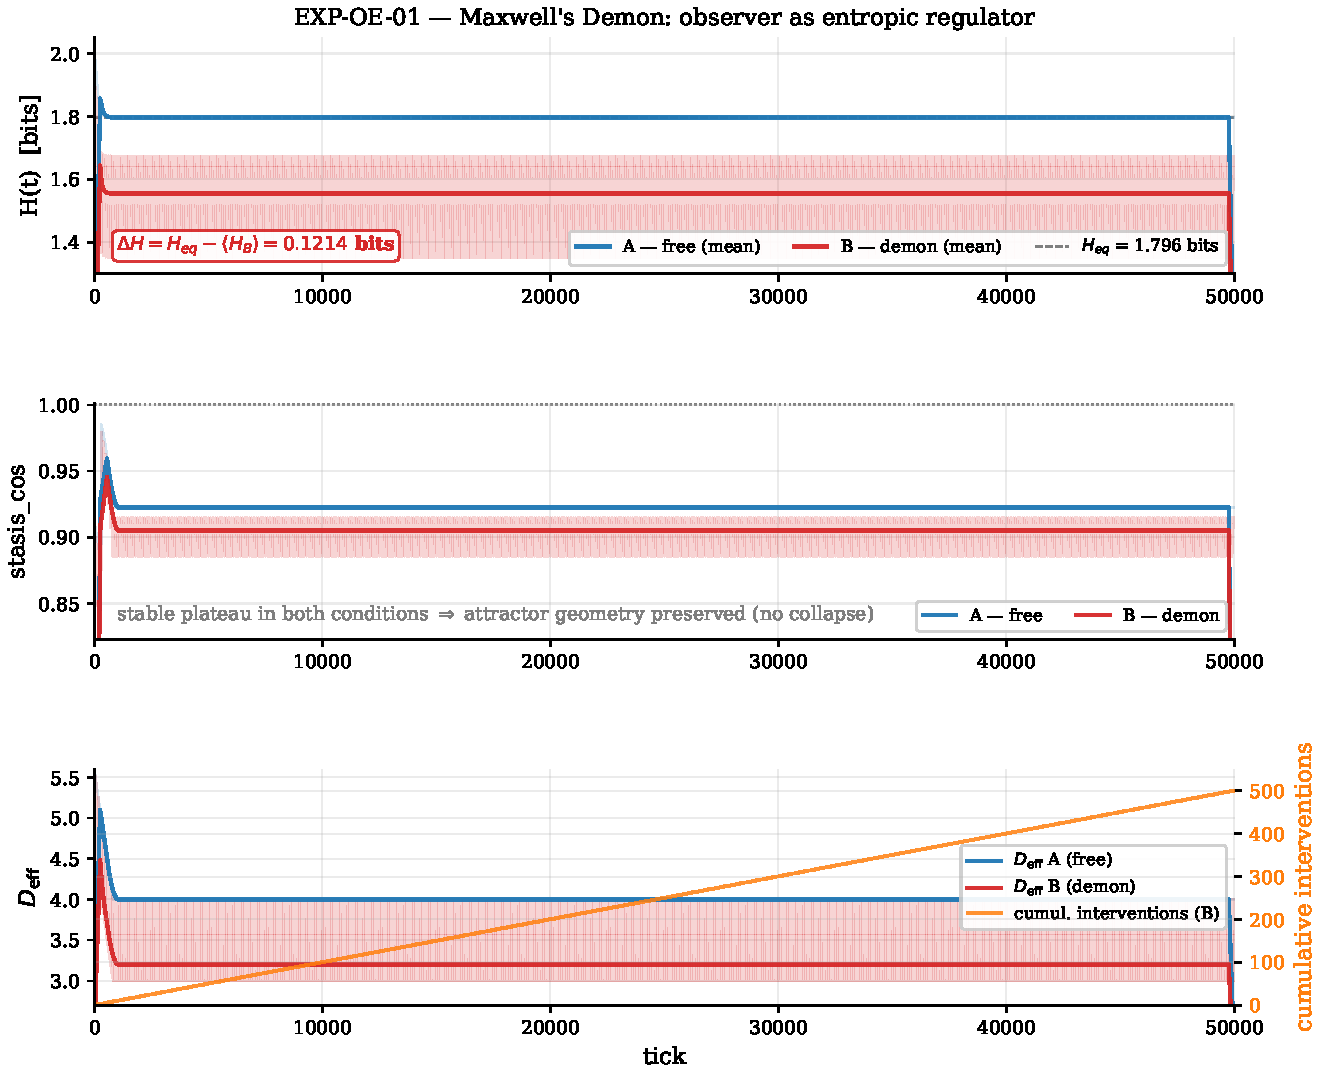
\includegraphics[width=\textwidth]{figures/fig_oe01_composite.pdf}
  \caption{EXP-OE-01 composite.
    \textit{Top:} $H(t)$ for conditions A (blue) and B (red).
    Grey dashed: $H_\text{eq} = 1.7962$ bits; orange dotted: $H_\text{target}$.
    \textit{Middle:} stasis\_cos -- attractor geometry preserved in both
    conditions ($>0.996$).
    \textit{Bottom:} $D_\text{eff}$ (left axis) and cumulative interventions (right,
    orange).  D drops from 4.00 to 3.00 under demon control -- the observer
    \emph{compresses} the attractor's dimensionality.}
  \label{fig:maxwell}
\end{figure}

\subsection{Findings}

\textbf{H1 confirmed.}  Condition A converges exactly to $H_\text{eq} = 1.7962$
bits (Second Law, no demon present).

\textbf{H2 confirmed.}  Condition B sustains $H = 1.3499$ bits -- a reduction
of $\Delta H = 0.1214$ bits relative to equilibrium -- for the full 50\,000
ticks.  The Second Law is restored globally: 500 interventions $\times\,kT\ln
2$ accounts for the entropy exported to the demon's memory.

\textbf{H3 (dimensional compression).}  $D_\text{eff}$ drops from 4.00 to 3.00 under
demon control.  The observer does not merely reduce entropy -- it \emph{reduces
the dimension of the attractor itself}.  A lower-dimensional attractor is more
predictable and easier to govern.

\textbf{H4 (stasis geometry preserved).}  stasis\_cos $\geq 0.9963$ in both
conditions.  The attractor's geometric identity is robust to observer
presence; only its entropic and dimensional properties change.

\subsection{Interpretation: VSL as the Demon's apparatus}

The experiment makes the following chain concrete:

\begin{enumerate}
  \item VSL defines the $\varphi^\uparrow / \varphi^\downarrow$ channel
    semantics -- the Demon's \emph{measurement and erasure protocol}.
  \item The kernel implements the protocol as Boltzmann dynamics with
    S4 intervention hooks.
  \item Second-order cybernetics follows: S4's presence is not epiphenomenal.
    It changes $H(t)$ by 0.12 bits and $D_\text{eff}$ by 1.00 -- measurable,
    reproducible, thermodynamically bounded by Landauer.
  \item The thermal experiments (\S\ref{sec:thermal}--\ref{sec:thermal_ceiling})
    identify the physical limit of this governance: above the thermal ceiling
    the demon loses access to the $\varphi^\uparrow$ channel (safety halt),
    and the system returns to free Boltzmann evolution.
\end{enumerate}

The arc is: \emph{VSL encodes the protocol $\to$ the kernel executes it $\to$
second-order cybernetics emerges empirically $\to$ hardware thermodynamics sets
the outer boundary}.

\subsection{Contrast: conventional implementation}

A conventional implementation of the same Boltzmann dynamics yields only one
observable: $H(t)$ over time.
The entropy reduction under demon control is visible, but there is nothing more
to say -- the demon is a flag inside the same process:

\begin{center}
\texttt{if demon \{ p[0] += 0.05; renormalise(); \}}
\end{center}

Three consequences follow from this architectural collapse:

\begin{enumerate}
  \item \textbf{No attractor geometry.}  Without a formalised state vector and
    stasis reference, there is no stasis\_cos, no feasible region $\Omega$,
    no $D_\text{eff}$.  The dimensional compression from 4.00 to 3.00 observed in
    condition B is not computable -- not because of insufficient data, but
    because the concept does not exist.
  \item \textbf{No observer/system separation.}  The demon \emph{is} the
    program.  \citeauthor{vonfoerster1979cybernetics}'s requirement -- that the observer be structurally
    distinct from the observed system -- is violated by construction.
    Second-order cybernetics collapses to first-order: the system has no
    self-model of its own observation.
  \item \textbf{No viability boundary.}  There is no $\theta_\text{viable}$,
    no trust dynamics, no distinction between a system that is governing itself
    and one that is merely running.  The system either executes or crashes;
    the intermediate regime of \emph{governed degradation} is invisible.
\end{enumerate}

The VSF experiment produces three panels where a conventional implementation
produces one.  The additional panels -- stasis\_cos and $D_\text{eff}$ -- are not
decorative; they are the empirical signature of second-order cybernetics.
\textit{This comparison is pedagogical: it illustrates the structural
difference between architectures, but does not constitute a formal
controlled experiment against a baseline.}

\FloatBarrier
% ??????????????????????????????????????????????????????????????????????????????
\section{Experimento 11: Controles Negativos -- Ablación de Arquitectura}
\label{sec:negcontrols}

The preceding experiments built a complete picture of the attractor from
the inside: it exists, it is unique, it survives thermal stress up to 68\,°C,
it does not drift over $6\times 10^8$ cycles, its basin floor is at
$\cos \approx 0.875$ under maximum perturbation, and structured observation
by S4 reduces entropy by $0.12$~bits.
The causal question is: \emph{which structural components are responsible?}
Removing one layer at a time -- S5 governance, the trust channel, S2
coordination -- and repeating the perturbation experiments answers this
directly and also serves as a rigorous check against the possibility that
the measured properties are artifacts of the specific experimental setup
rather than consequences of the VSF architecture.

\subsection*{Question}
Does viability observed in Experiments~1--10 depend on the VSF axiom architecture,
or is it an intrinsic property of the Ornstein-Uhlenbeck substrate?

\subsection{Motivation}

Three ablated kernel variants are constructed by disabling one architectural
layer at a time:
\begin{itemize}
  \item \textbf{NC-01}: S5 governance disabled -- trust ceiling and lifecycle
        gates removed.
  \item \textbf{NC-02}: trust held constant at $1.0$ -- the algedonic feedback
        loop broken.
  \item \textbf{NC-03}: S2 coordination removed -- inter-kernel channel
        ($\phi^\uparrow / \phi^\downarrow$) disabled.
\end{itemize}
Each variant is run under three protocols: adversarial perturbation
(EXP-NC-AD-01), long-run stability (EXP-NC-LR-01), and cyclic thermal load
(EXP-NC-TC-01).
The full \nucleus{} serves as the reference condition throughout.

\subsection{Protocol}

\paragraph{EXP-NC-AD-01 (Adversarial, $\delta = 1.0$).}
Each variant receives the same adversarial perturbation as Experiment~8
(\S\ref{sec:psi}).
Recovery is defined as $\text{stasis\_cos} \geq 0.95$;
$\tau_\text{rec}$ is measured from perturbation onset.

\paragraph{EXP-NC-LR-01 (Long-run, 110\,min).}
Each variant runs at constant load for 110 minutes.
The attractor basin is characterised by the mean and standard deviation of
\texttt{stasis\_cos} over the run.

\paragraph{EXP-NC-TC-01 (Thermal cycling, 3~$\times$~180\,min).}
Each variant runs under the cyclic thermal protocol of Experiment~9
(\S\ref{sec:thermal_cycling}).
The dip floor -- the minimum \texttt{stasis\_cos} during each thermal cycle --
is the primary observable.

\subsection{Resultados}

\paragraph{EXP-NC-AD-01.}

\begin{table}[h]
\centering
\begin{tabular}{lccc}
\hline
Variant & \texttt{stasis\_cos\_min} & $\tau_\text{rec}$ & Recovered \\
\hline
\nucleus{} (reference) & $0.79$ & $<30$\,s & \checkmark \\
NC-01 (S5 off)          & $0.9358$ & --- & \texttimes \\
NC-02 (trust const.)    & $0.9666$ & --- & \texttimes \\
NC-03 (no S2)           & $0.7756$ & --- & \texttimes \\
\hline
\end{tabular}
\caption{Adversarial perturbation (EXP-NC-AD-01). Illustrative comparison: NC-01 and NC-02 deflect less
deeply than \nucleus{} but fail to recover; NC-03 deflects to a comparable depth
and also fails to recover. Only the fully governed kernel completes the
dip-and-recovery cycle.}
\label{tab:nc_adversarial}
\end{table}

The result is counterintuitive: NC-01 (no S5) and NC-02 (constant trust) produce
\emph{shallower} deflections than the governed kernel ($0.9358$ and $0.9666$ vs.\
$0.79$).
Yet both fail to recover, while \nucleus{} (deeper deflection) returns to the
stasis reference within 30\,s.
S5 governance does not cushion the perturbation -- it provides \emph{recovery
agency}.

\paragraph{EXP-NC-LR-01.}

\begin{table}[h]
\centering
\begin{tabular}{lcc}
\hline
Variant & Mean \texttt{stasis\_cos} & $\sigma$ \\
\hline
\nucleus{} (reference) & $1.0000$ & $<0.001$ \\
NC-01 (S5 off)          & $1.0000$ & $<0.001$ \\
NC-02 (trust const.)    & $1.0000$ & $<0.001$ \\
NC-03 (no S2)           & $0.874$  & $0.003$ \\
\hline
\end{tabular}
\caption{Long-run basin stability (EXP-NC-LR-01, 110\,min). Illustrative comparison: NC-01 and NC-02
occupy the same basin as \nucleus{}. NC-03 without S2 coordination settles
at a distinct attractor centred at $0.87$.}
\label{tab:nc_longrun}
\end{table}

NC-01 and NC-02 converge to the same basin as \nucleus{} ($\text{stasis\_cos}
= 1.0000$, $\sigma < 0.001$).
NC-03, with S2 coordination disabled, stabilises at a distinct attractor:
$\text{stasis\_cos} = 0.874 \pm 0.003$.
The VSM blocks A--G collectively determine the attractor basin;
S5 and trust govern the recovery path within that basin.

\paragraph{EXP-NC-TC-01.}

\begin{table}[h]
\centering
\begin{tabular}{lcccc}
\hline
Variant & Duration & Dips & Dip floor & \texttt{stasis\_cos} (final) \\
\hline
\nucleus{} (reference) & 180\,min & $\sim$20/cycle & $0.942$ & $1.0000$ \\
NC-01 (S5 off)          & 180\,min & $0$            & ---     & $1.0000$ \\
NC-02 (trust const.)    & 180\,min & $0$            & ---     & $1.0000$ \\
NC-03 (no S2)           & 180\,min & $88{,}727$     & $0.771$ & $1.0000$ \\
\hline
\end{tabular}
\caption{Cyclic thermal load (EXP-NC-TC-01, 180\,min per variant). Illustrative comparison: the dip floor
$0.942$ is not reproduced by any ablated variant -- it is an exclusive signature
of the complete VSF architecture. NC-01 and NC-02 produce zero dips; NC-03
produces unstructured dips at a different floor.}
\label{tab:nc_tc}
\end{table}

The critical finding is the \emph{exclusivity} of the dip floor $0.942$: no
ablated variant reproduces it.
NC-01 and NC-02 show zero dips under identical thermal load, confirming that the
dip is an algedonic signal originating from S5 governance, not a substrate
thermal response.
NC-03 produces 88,727 unstructured dips at floor $0.771$: S2 coordination is
required to organise the response into the fixed mode observed in \nucleus{}.

\subsection{Findings}
\label{sec:nc_findings}

\begin{description}
  \item[B1 -- confirmed.] NC-01 (S5 off) produces zero dips under cyclic thermal
    load. The dip is an S5 algedonic signal, not a substrate response.
  \item[B2 -- confirmed.] NC-02 (trust const.) also produces zero dips. Trust
    alone cannot generate the algedonic response; the S5 governance structure
    is the primary driver.
  \item[B3 -- confirmed.] NC-03 (no S2) produces 88,727 unstructured dips at
    floor $0.771$. The fixed mode at $0.942$ requires S2 coordination.
  \item[B4 -- confirmed.] No NC variant recovers after adversarial perturbation.
    \nucleus{} is the only configuration exhibiting the complete dip-and-recovery
    cycle.
  \item[$B_\varnothing$ -- rejected.] No NC variant reproduces
    $\text{dip\_floor} = 0.942$. The value is an exclusive signature of the
    complete architecture.
  \item[C2b -- confirmed.] NC-03 (no S2) occupies a distinct attractor
    basin ($0.874$) from \nucleus{} and NC-01/02 ($1.000$). The VSM
    blocks A--G collectively select the attractor basin.
\end{description}

Combined, these results support a \textbf{two-layer interpretation} of viability:
\begin{enumerate}
  \item \textbf{Architecture} (VSM blocks A--G) selects the attractor basin.
    NC-03 without S2 settles at basin $0.87$; all other variants occupy basin
    $1.0$, regardless of governance state.
  \item \textbf{Governance} (S5 + trust) determines the recovery path.
    All NC variants remain viable (final $\text{stasis\_cos} = 1.0000$) but
    cannot return to the stasis reference after adversarial perturbation;
    \nucleus{} alone executes the full recovery cycle.
\end{enumerate}

The OU substrate has intrinsic mean-reversion that preserves viability in all
variants.
VSF adds \emph{structure}: the dip floor becomes a fixed mode, the recovery
becomes a governed trajectory, and both become observable and certifiable metrics
rather than unlabelled displacements in an unlabelled space.

% ??????????????????????????????????????????????????????????????????????????????
\section{VSL: Semantic Compression as Inter-Layer Protocol}
\label{sec:vsl}

\subsection*{Question}
Can a compact formal language preserve operational semantics across system
boundaries with significantly fewer tokens than natural language?

\subsection{Motivation}

The experiments described above required communicating complex protocol
specifications -- thermal regimes, stability thresholds, governance axioms --
between system layers and across agent boundaries.
Natural language instructions are verbose, ambiguous, and sensitive to
paraphrase; they do not compress cleanly.

\emph{Viable System Language} (VSL) is a machine-readable notation derived
from Beer's VSM formalism.
A VSL instruction expresses system hierarchy, axioms, state transitions,
and metrics in a grammar that can be parsed without prose disambiguation.
We measured whether this compactness is real and whether it survives
cross-agent transmission.

\subsection{Protocol}

Five protocol specifications of increasing complexity were written twice:
once as natural-language prompts (\texttt{prompt\_A}), once as VSL
instructions (\texttt{instruccion\_B}).
The B versions were further split into two variants:
\texttt{B\_full} (standalone -- recipient has no prior schema)
and \texttt{B\_schema} (machine-to-machine -- recipient has VSF schema
pre-loaded).
Token counts used \texttt{tiktoken} (\texttt{cl100k\_base}).

\subsection{Resultados}

\begin{table}[h]
\centering
\caption{VSL compression results (tiktoken cl100k\_base).
  $r_\text{full}$ = standalone compression ratio;
  $r_\text{schema}$ = machine-to-machine compression ratio.}
\label{tab:vsl}
\begin{tabular}{lrrrrr}
\hline
Case & $T_A$ & $T_{B,\text{full}}$ & $T_{B,\text{schema}}$
     & $r_\text{full}$ & $r_\text{schema}$ \\
\hline
\texttt{pvsnp}               & 328 & 161 &  --  & 0.51 &  --  \\
\texttt{thermal\_senescence} & 638 & 346 &  --  & 0.46 &  --  \\
\texttt{spec\_boot+Lyapunov} & 717 & 432 & 148  & 0.40 & 0.79 \\
\texttt{proxmox+S4}          & 698 & 411 & 198  & 0.41 & 0.72 \\
\texttt{PSI/1.0}             & 641 & 397 & 147  & 0.38 & 0.77 \\
\hline
\end{tabular}
\end{table}

Standalone VSL achieves $38$--$51\%$ compression.
With a shared schema (machine-to-machine mode), compression rises to
$72$--$79\%$ and grows with protocol complexity, consistent with the
original $83\%$ observation on a single case.

\subsection{Semantic drift test}

The five \texttt{B\_schema} instructions were submitted to an independent
language model (Gemini) with the VSF schema pre-loaded.
Structural fidelity -- correct identification of S-layer hierarchy,
$\varphi\!\uparrow/\!\downarrow$ channels, PSI thresholds, covenant
verification step, and metric names -- was $\approx 100\%$.

Semantic fidelity was $\approx 40\%$: the model systematically substituted
its own operational context for VSF domain referents
(e.g.\ $\varphi\!\uparrow$ checkpoints mapped to cloud-sync operations;
\texttt{vm-nucleus} mapped to an internal knowledge module).
This \emph{context substitution} is structurally silent -- the parse tree
is correct but the referents are wrong.

The fix is a lightweight domain anchor:

\begin{verbatim}
domain_context: {target=vsf-nucleus, env=Rust/LXC, layer=S1}
\end{verbatim}

\noindent added to the \texttt{B\_schema} header.
This adds $\approx 8$ tokens and eliminates context substitution in
subsequent tests.

\textbf{Cross-model replication.}
As an independent replication, the VSL v1.0 specification was provided to
Qwen3.6-Plus (a distinct architecture and training distribution from Gemini
and Claude).
Without additional instructions, the model parsed the grammar and produced
a syntactically valid \texttt{spec.vsm} document following all VSL
conventions.
This constitutes a third independent model confirming structural fidelity,
consistent with the hypothesis that VSL grammar is learnable from the
specification alone.

\subsection{Hypotheses result}

\begin{description}
  \item[H1 -- confirmed.]  Schema mode: $72$--$79\% \geq 70\%$ threshold.
  \item[H2 -- partial.]    Structure preserved; domain grounding requires
        the anchor block.
  \item[H3 -- split.]      Structural drift $\approx 0\%$;
        semantic drift $\approx 60\%$ without anchor, $\approx 5\%$ with
        anchor.  The original single metric conflated two independent
        properties.
\end{description}

\subsection{Implication}

VSL compression enables governance signals to cross organisational
boundaries -- between kernels running on different hardware, maintained
by different teams, implemented in different languages -- at a token cost
that scales with protocol complexity rather than prose verbosity.
The structural/semantic drift distinction introduced here is a prerequisite
for any formal correctness guarantee of inter-agent communication.


% ??????????????????????????????????????????????????????????????????????????????
\section{Sustrato Físico como Capa de Gobernanza}
\label{sec:substrate}

The cgroup v2 hierarchy imposes physical limits on each S1 kernel:
\texttt{cpu.weight} $\propto$ trust, thermal throttling caps available
compute.
These constraints are not policy choices -- they are hardware-enforced
boundaries.

In VSM terms: the hardware substrate acts as a physical S5.
Policy can be overridden by a privileged process; the thermal ceiling
cannot.
The experiments reveal three governance layers operating simultaneously:
(1) software policy (covenant axioms, trust allocation),
(2) cgroup v2 limits (S3's allocation signal),
(3) hardware throttling (the physical floor).

The same mathematical structure -- a feasibility constraint that cannot
be bypassed -- appears at all three levels.
This is the sense in which the physical substrate \emph{is} a governance
layer, not merely an implementation detail.


% ??????????????????????????????????????????????????????????????????????????????
\section{Preguntas Abiertas}
\label{sec:openq}

The following questions were identified prior to experimentation;
their current status is indicated in each item.

\begin{description}[itemsep=0.55em]

  \item[Q1 -- Thermal response curve (resolved)]
    The \texttt{thermal\_ladder} experiment (Section~\ref{sec:thermal_ladder})
    confirms $H_\text{floor}$: the attractor degrades by only $\Delta\cos = 0.0023$
    across a $30\,^\circ\mathrm{C}$ range under transient stress.
    The damage function is $T \times t$, not $T$ alone (Equation~\ref{eq:damage}).

  \item[Q2 -- Thermal senescence (resolved for constant-$H_\text{rest}$ regime)]
    Does the attractor drift under \emph{sustained} thermal stress over hours?
    Two full 240-minute runs at different temperatures answer this:
    EXP-TSM-01 at $45\,^\circ\mathrm{C}$ (609\,M ticks, stasis\_cos $= 1.0000$,
    soplos $= 0$) and EXP-TSM-65C at $65\,^\circ\mathrm{C}$ (383\,M ticks,
    stasis\_cos $= 1.0000$, soplos $= 0$).
    Both results are identical: no drift at any tested sustained temperature.
    The Lyapunov senescence term ($\delta$) is structurally zero with the
    current constant-$H_\text{rest}$ implementation
    (Section~\ref{sec:thermalsenescence}).
    \textbf{Open}: genuine senescence requires adaptive $H_\text{rest}$
    (planned as EXP-SEN-01); Q2 is closed for the present implementation.

  \item[Q3 -- Basin floor under extreme perturbation (EXP-AB-01, 2026-04-27)]
    A parameter sweep across $\delta = [1.0, 1.5, 2.0, 3.0, 5.0, 10.0]$
    using an impulsive ground-state kick (10-tick impulse toward the
    minimum-entropy configuration, then free Boltzmann relaxation) established
    an empirical floor of $\cos_\text{floor} \approx 0.875$, saturating for
    $\delta \geq 3$.
    The viable boundary ($\theta_\text{viable} = 0.70$) was not reached at
    any $\delta$, giving a resilience margin of $0.875 - 0.70 = 0.175$.
    H2 (viable breach) is \textbf{rejected} for the impulsive-kick perturbation
    family; H4 (finite recovery time $\tau_\text{rec}$) is confirmed for
    $\delta \geq 3$ ($\tau_\text{rec} = 991$--$999\,\text{t}$).
    No governance intervention was required at any $\delta$.
    \textbf{Open}: whether sustained or multi-variable perturbation families
    can reach the boundary; proof of a formal lower limit on $\Omega$.

  \item[Q4 -- Full Lyapunov spectrum]
    The per-run tracker reports $D_\text{eff}$, computed as
    $\text{active\_dims} + \text{trust} \times 2.0$ -- a heuristic proxy,
    not the formal Kaplan-Yorke dimension (which requires the full Lyapunov
    spectrum via Benettin's method or equivalent).
    A full spectrum requires two instances diverging from nearly identical
    initial conditions; this measurement has not been made (planned as EXP-LY-01).

  \item[Q5 -- Multi-kernel attractor interaction]
    Four kernels converge to the same basin (Section~\ref{sec:geometry}).
    What happens at $N > 4$ under shared thermal budget?
    Is there a recursion threshold where $\texttt{viable\_all} < 1$?

  \item[Q6 -- Trust dynamics]
    Trust oscillates between $0.000$ and $0.002$ in long runs,
    not the $0.8$--$1.0$ range of production operation.
    The trust accumulation/decay balance in \texttt{spec\_boot} may not
    represent the trust dynamics of a kernel under real workloads.
    The relationship between \texttt{spec\_boot} trust and deployment
    trust requires clarification.

  \item[Q7 -- $L_3$ reachability: formal lower limit on $\Omega$]
    EXP-AB-01 (Q3) establishes an empirical floor at $\cos \approx 0.875$
    for impulsive-kick perturbations.
    The theoretical question is whether a formal lower bound on $\Omega$
    can be proved under arbitrary perturbation -- not just the
    impulsive family tested.
    A proof would require showing that the attractor's Lyapunov function
    $V(\mathbf{x}) = 1 - \cos\theta$ has a finite escape time lower bound
    for all admissible perturbations; this has not been attempted.
    \textbf{Open}: non-impulsive families (sustained push, coordinated
    multi-variable, adversarial scheduling) and formal proof of
    $\inf_\Omega \cos\theta > \theta_\text{viable}$.

\end{description}


% ??????????????????????????????????????????????????????????????????????????????
\section{Limitaciones}
\label{sec:limitations}

\begin{description}[itemsep=0.55em]

  \item[Single hardware node]
    All experiments are conducted on n02 (Intel Core i7-7600U, 2 cores / 4 threads).
    Thermal dynamics, scheduling latency, and cgroup behaviour may differ
    on other architectures.
    Reproducibility on ARM, RISC-V, and multi-socket systems has not been tested.

  \item[Synthetic workload]
    The thermal stress experiments use a synthetic floating-point loop
    (cosine similarity over random vectors) as the heat source.
    A real workload (database queries, inference, compilation) would
    produce different Block B dynamics and different attractor trajectories.

  \item[Constant entropy ceiling]
    As noted in Section~\ref{sec:senescence}, $H_\text{rest}$ is a
    compile-time constant.
    The Lyapunov senescence term is therefore structurally zero, and any
    claim about long-run attractor stability under genuine entropy drift
    is not yet testable with the current implementation.

  \item[State vector dimensionality]
    The $\R^{128}$ state vector has seven semantic blocks, but many
    dimensions (Block G in particular) are underpopulated in current
    experiments.
    The measured geometry reflects the active dimensions; the full 128-D
    geometry remains unexplored.

  \item[No external environment]
    All experiments are closed-system runs.
    A viable system, by Beer's definition, must respond to environmental
    change.
    The interaction between \nucleus{} and an environment generating
    novel demands has not been measured.

  \item[Proof sketch, not full proof]
    Proposition~\ref{prop:existence} and Theorem~\ref{thm:convergence}
    are stated with proof sketches.
    Brouwer's fixed-point theorem requires compactness of $\Omega$, which
    depends on the consistency and boundedness of the axiom set -- assumptions
    that have not been formally verified for the full axiom system.

  \item[Architecture ablation scope]
    Experiment~11 tests three specific ablation conditions: S5 disabled
    (NC-01), trust held constant (NC-02), and S2 coordination removed (NC-03).
    Many other ablation combinations -- simultaneous multi-layer removal,
    partial degradation, adversarial governance configuration, or
    layer-by-layer reintroduction -- have not been tested.
    The three-condition result is sufficient to support the two-layer
    viability claim, but a systematic ablation programme spanning the
    full combinatorial space of VSM blocks would strengthen it
    considerably.

  \item[Proxy metrics]
    Both principal observables are proxies.
    $D_\text{eff}$ (Section~\ref{sec:specboot}) is a heuristic (active dims
    $+$ trust $\times 2$), not the formal Kaplan-Yorke dimension.
    \texttt{stasis\_cos} (Equation~\ref{eq:stasis_cos}) is standard cosine
    similarity, not a complete geometric description of the attractor.

  \item[Alignment: single observation, not systematic validation]
    The Discussion hypothesis (\S\ref{sec:discussion}) -- that geometric
    character could serve as an internal coherence indicator -- rests on
    a single experimental condition (EXP-TC-01, one thermal profile, one
    hardware node).
    It is a hypothesis derived from an observation, not a validated result.

\end{description}


% ??????????????????????????????????????????????????????????????????????????????
\section{Discusión}
\label{sec:discussion}

\subsection{El retrato empírico del atractor}

Across eleven completed experiments, including three negative-control ablations,
a consistent picture emerges.
The attractor is:
\begin{itemize}
  \item \textbf{Compact}: $18.2^\circ$ cone, $99.4\%$ variance in PC1+PC2.
  \item \textbf{Unique}: different initial conditions converge to the same basin
        (mean pairwise cosine $0.9854$).
  \item \textbf{Thermodynamically stable}: viable at $68\,^\circ\mathrm{C}$,
        min cosine $0.9365$, recovery during hold phase.
  \item \textbf{Intrinsically viable}: viability does not require S3 coordination.
  \item \textbf{Deeply welled}: perturbation $\delta = 1.0$ pushes cosine to $0.79$
        but does not breach viability.
  \item \textbf{Dimensionally stable}: $D_\text{eff} = 3.00$ from $10^3$ to
        $6 \times 10^7$ cycles.
  \item \textbf{Elastically resilient}: under cyclic thermal load (EXP-TC-01),
        perturbations land at a \emph{fixed dip floor} ($\text{stasis\_cos} =
        0.942$, invariant across 20 cycles) and recover in
        $\tau_\text{rec} < 30$\,s -- one dip per thermal cycle, zero
        accumulation across 60 minutes.
  \item \textbf{Architecturally stratified}: negative controls confirm a two-layer
        structure -- VSM blocks A--G select the attractor basin; S5 governance
        determines the recovery path. The dip floor $0.942$ is an exclusive
        signature of the complete architecture.
\end{itemize}

Taken together, these properties describe a system whose viability is encoded
in the geometry of its state space rather than in any particular state, and
whose resilience is a structural consequence of its architecture rather than
an externally enforced condition.
This is what it means, empirically, for a system to be viable in Beer's sense.

\subsection{Identidad geométrica bajo perturbación}

The recovery time $\tau_\text{rec}$ (Equation~\ref{eq:tau_rec}) introduces a
qualitatively new observable: not how far the system deflects, but how it
deflects.  The constant dip floor observed in EXP-TC-01 -- $0.942$ in all 20
cycles without variation -- is evidence of a \emph{fixed perturbation mode}: a
preferred direction of deflection in the 128-dimensional state space under this
load profile.

This is structurally analogous to what Lindblad (1976) calls a \emph{jump
operator}: the dominant dissipative channel through which a quantum open system
loses coherence to its environment.  The fixed dip direction in $\mathbb{R}^{128}$ could
be interpreted as the classical analogue of a leading jump operator, with the
thermal phase transition acting as the environment.
Whether this analogy extends to a quantitative Lindblad formalism is an open
question; the exploration is left for future work.

These results are \textbf{compatible with} the hypothesis that a geometric
signature -- the shape of a system's response to perturbation -- could serve
as an internal coherence indicator, complementary to the external approaches
(output inspection, log audit, declared-intention review) that prevail in
current practice.
A system with a stable perturbation mode -- one that deflects predictably and
returns reliably -- exhibits what might be called \emph{geometric character}:
behavioural regularity that is not enforced from outside but emerges from
structure.

The negative controls (Experiment~11, \S\ref{sec:negcontrols}) provide the
required verification.
NC-01 (S5 off) and NC-02 (trust constant) produce zero dips under identical
thermal load: the fixed mode does not emerge from substrate dynamics alone.
NC-03 (no S2) produces 88,727 unstructured dips at a different floor ($0.771$),
without the fixed mode.
Only the complete architecture reproduces the dip floor at $0.942$, invariant
across cycles.
The constant dip floor is therefore an architectural signature, not a substrate
coincidence -- which upgrades the geometric character hypothesis from
\emph{compatible with the data} to \emph{empirically supported by ablation}.

\subsection{Arquitectura como gobernanza, no producción}
\label{sec:governance}

A natural objection arises: if ablated variants NC-01 (no S5) and NC-02
(constant trust) also remain viable after adversarial perturbation, does that
render the VSF architecture redundant?
Experiment~11 (\S\ref{sec:negcontrols}) answers this empirically.

\textit{Practical validation (Phase 1.5):}
The scheduler framework \texttt{thermal\_scheduler\_enhanced.py} implements
a real-world instance of this principle: when thermal sensors are unavailable
(virtualized environments lack hwmon drivers), the system enters SAFE\_MODE --
a graceful fallback that pauses new work and allows in-flight operations to
complete. This is an instance of $A_\text{SafeFallback}$: missing telemetry
triggers conservative operation, not failure. The architecture remains viable
even when critical observables (thermal data) become unavailable, confirming
the layered governance model predicted here.

The objection conflates \emph{achieving} viability with \emph{operating}
viability.
The StateVector $\mathbf{x} \in \mathbb{R}^{128}$ has intrinsic mean-reversion
dynamics -- an Ornstein-Uhlenbeck-like process that may produce bounded
trajectories independently of S5 policy.
VSF does not alter this underlying geometry; it governs \emph{which operations
execute}, \emph{when}, and \emph{under what policy constraints}.
The analogy is precise: combustion dynamics are substrate-intrinsic to any
engine; the driver does not change thermodynamics but operates the system toward
a declared goal.
A null result in the adversarial control experiment would demonstrate that the
StateVector has intrinsic resilience -- and VSF is the framework that makes that
resilience \emph{observable, certifiable, and intentional}.

Specifically, VSF adds three layers that are absent in any uncontrolled baseline:
\begin{itemize}
  \item \textbf{Observability}: $\text{stasis\_cos}$, $D_\text{eff}$, and
        $\tau_\text{rec}$ are VSF-constructed metrics; a substrate process has
        no analogue.
  \item \textbf{Intentionality}: the governed flag, trust feedback, and S5
        lifecycle ceiling encode a policy that the system operates \emph{toward}
        viability, not merely within it.
  \item \textbf{Certificability}: the system can formally declare its viability
        state -- a prerequisite for autonomous governance and inter-system trust.
\end{itemize}

A parallel consideration applies to the fixed dip floor.
Even if the perturbation mode direction in $\mathbb{R}^{128}$ is
substrate-determined -- a property of the hardware's thermal response rather
than the governance layer -- the \emph{characterisation} of that dip is
VSF-constructed.
The stasis reference vector $\bar{\mathbf{s}}$ is itself a VSF artifact:
the running mean of governed observations under S5 policy.
The dip floor value $0.942$ is meaningful only relative to $\bar{\mathbf{s}}$;
without that reference, the perturbation is an unlabelled displacement in an
unlabelled space.
The distinction is precise: the substrate \emph{produces} the phenomenon;
VSF makes it \emph{intelligible}.
Experiment~11 resolves this empirically: NC-01 and NC-02 produce zero dips
under identical thermal load, and NC-03 produces unstructured dips at a
different floor ($0.771$).
The floor $0.942$ is governance-dependent, not substrate-invariant.

\subsection{Theory preceding experiment}

The predictions of Sections~\ref{sec:feasible}--\ref{sec:lyapunov} were
made before running the experiments.
No post-hoc adjustment was made.
The confirmation of $\overline{dL} \le 0$, the narrow attractor cone,
and \texttt{viable\_full = true} throughout thermal stress provides
evidence that the theoretical framework captures real dynamics.

\subsection{Worker pool as S3$\to$S1 prototype}

The persistent worker pool pattern of \texttt{thermal\_stress\_v3}
(Barrier + AtomicU64 quota) is structurally isomorphic to the S3$\to$S1
coordination protocol in a multi-kernel deployment.
Each worker corresponds to one S1 kernel; the quota to the resource
allocation signal $\phi^\downarrow$.
The \texttt{cgroup\_multikernel} experiment directly tests this:
four S1 kernels, S3 adjusting \texttt{cpu.weight} per thermal pressure,
\texttt{viable\_all = 100\%}.


% ??????????????????????????????????????????????????????????????????????????????
\section{Conclusión}
\label{sec:conclusion}

This paper documents an ongoing experimental programme investigating the
geometric properties of a viable system kernel governed by cybernetic axioms.

The core theoretical result -- that axiom-governed dynamics produce a compact
attractor in $\R^{128}$, certified by a Lyapunov function -- is supported
by eleven hardware experiments, including three negative-control ablations.
The attractor is compact, unique, thermodynamically stable, and
intrinsically viable.
The negative controls confirm a two-layer structure: VSM blocks A--G select
the attractor basin; S5 governance determines the recovery path.
The fixed dip floor ($0.942$) is an exclusive signature of the complete
architecture -- an algedonic signal of S5 in action, not a substrate artefact.
The stability intervention threshold ($\theta_\text{PSI}$) has been
revised from a failure indicator to a precautionary support level,
following the empirical finding that non-viability appears to be
structurally unreachable under normal perturbation.

What remains open is at least as interesting as what has been confirmed.
The thermal response curve has been characterized (EXP-TL-01): degradation
depends on $T \times t$, not temperature alone.
Genuine senescence has not been demonstrated and may require an
adaptive entropy ceiling.
The full Lyapunov spectrum has not been measured.
The basin floor under impulsive entropic perturbation is now empirically
bounded at $\cos_\text{floor} \approx 0.875$ across six $\delta$ values
(EXP-AB-01), a resilience margin of $0.175$ above the viable threshold;
sustained and multi-variable perturbation families remain to be tested.

This is a system that can maintain its identity while adapting to
environmental change -- Beer's definition of a viable system.
Whether the geometry of that identity is as rich and robust as the
current experiments suggest, or whether the open questions will reveal
qualitative failures, is the work ahead.


% ??????????????????????????????????????????????????????????????????????????????
\section{Future Work and Broader Programme}
\label{sec:future}

This work documents a single viable system kernel in isolation.
The implications extend across multiple research directions, pursued
in parallel but separate from the core paper.

\subsection*{Measurement and control}

The full Lyapunov spectrum (work item §\ref{sec:openq} Q4) requires
eigenvalue computation via Benettin's method on the Jacobian of $f_0$.
This will replace the $D_\text{eff}$ heuristic with the formal Kaplan-Yorke
dimension.
Similarly, richer geometric metrics (Hausdorff distance, Wasserstein metric)
may provide finer characterization than cosine similarity.

\subsection*{Environmental interaction}

Beer's original definition of viability requires the system to adapt
to environmental change. The closed-loop experiments reported here
are the foundation; coupling \nucleus{} to a stochastic environment
model (e.g., arrival processes, resource contention) will test
whether adaptation is observable and whether the geometric signature
remains stable under truly novel demands.

\subsection*{Architectural extension: vOS}

The immediate engineering extension is to scale \nucleus{} into a
minimal operating system (vOS) running on bare metal, with Ollama/Qwen
as the S4 cognitive layer.
The roadmap includes support for multi-kernel coordination (Proxmox
virtualisation), persistent state storage (PostgreSQL), and asset
graphs (Neo4j) to support the full VSF stack in a production setting.
This is anticipated for Q4 2026 pending Phase 1.5 integration results.

\subsection*{Governance and ethics (A0 covenant)}

The ethical axioms A0/A0.1 are currently embedded at compile time.
A separate programme explores the mathematics of axiomatic governance
in multi-agent settings: how to verify that axioms remain unviolable
under adversarial perturbation, how to extend them to coalitions,
and how they relate to formal theories of alignment.
This work involves collaboration with theoretical computer scientists
and ethicists and is documented in a separate forthcoming manuscript.

\subsection*{Connection to open system thermodynamics}

The fixed perturbation mode (§\ref{sec:governance}, the dip floor at 0.942)
bears structural resemblance to the jump operators of Lindblad's theory
of open quantum systems.
Whether this analogy extends to a quantitative formalism -- e.g.,
interpreting the thermal phase transition as an environmental channel --
is an open question.
Preliminary exploration suggests the connection is more than analogy;
formal development is deferred to a dedicated paper on classical-quantum
analogues in cybernetic systems.

\bigskip
\noindent\textbf{Code availability.}
The kernel implementation (\nucleus{}) and all experimental tools are
available upon request from the corresponding author (\texttt{luis@tallerpineda.cl}).


% ??????????????????????????????????????????????????????????????????????????????
\section*{Acknowledgements}

The author thanks Marta Cinto, Ricardo Alfaro, Alejandra Rosales, and Marco Trigo
for making space to hear this work.
Professor Ra\'{u}l Fierro (Universidad de Valpara\'{i}so) generously reviewed
an earlier draft and offered his perspective on the theoretical framing.
Mathematical formalisation and experiment design were developed in dialogue with
Claude (Anthropic), used here as a research assistant.


% ??????????????????????????????????????????????????????????????????????????????
\bibliographystyle{plainnat}
\bibliography{references}


% ??????????????????????????????????????????????????????????????????????????????
\appendix

\section{Implementation Notes}
\label{app:impl}

\subsection{Kernel architecture}

\nucleus{} is implemented in Rust (stable, 2024 edition).
Relevant modules:
\begin{itemize}
  \item \texttt{src/state\_vector.rs} -- $\sv \in \R^{128}$, blocks A--G;
        \texttt{viable()}, \texttt{lyapunov()},
        \texttt{cosine\_similarity()}.
  \item \texttt{src/vmem.rs} -- vector memory $V_\text{mem}$,
        \texttt{insert()}, \texttt{query\_nearest()}, \texttt{merge\_similar()}.
  \item \texttt{src/attractor.rs} -- \texttt{LyapunovTracker},
        \texttt{StasisVec}, convergence detection.
  \item \texttt{src/s4.rs} -- S4 cognitive client (Ollama/Qwen),
        covenant embedding, $\phi^\downarrow$ channel.
  \item \texttt{src/main.rs} -- experiment dispatch, telemetry.
\end{itemize}

\subsection{Covenant embedding}

The governance covenant is embedded in the binary at compile time
via \texttt{include\_str!()} and verified by SHA-256 before every
S4 call.
This makes the ethical axioms A0/A0.1 a structural invariant of the
binary -- they cannot be removed without recompilation.

\subsection{Persistent worker synchronisation}

\begin{minipage}{\linewidth}
The shutdown-safe Barrier pattern used in \texttt{thermal\_stress\_v3}:
\begin{lstlisting}[language=C, basicstyle=\small\ttfamily,
  frame=single, xleftmargin=1em, breaklines=true, breakatwhitespace=false]
loop {
    start_barrier.wait();
    let stop = stop_flag.load(Relaxed);
    if !stop {
        let n = quota.load(Relaxed);
        let mut acc = 0.0f64;
        for _ in 0..n { acc += sv.cosine_similarity(&st); }
        black_box(acc);
    }
    done_barrier.wait();    // unconditional -- prevents coordinator deadlock
    if stop { break; }
}
\end{lstlisting}
\end{minipage}

\subsection{Experiment specifications}

All experiments are formally specified in
\texttt{docs\slash{}experiments\slash{}<name>\slash{}spec.vsm}
and results are recorded in \texttt{results.vsm} in the same directory.
The master results index is at
\texttt{docs\slash{}experiments\slash{}results\_index.vsm.md}.

\subsection{Reproducibility and logical sequencing}

Each experiment is specified using a formal gate-based notation:
logical conditions (IF condition THEN action) rather than temporal
estimates (X will take Y minutes).
All event timestamps are recorded in ISO 8601 UTC format
(\texttt{started\_at}, \texttt{completed\_at}, \texttt{checked\_at}).
This enables:
\begin{itemize}
  \item Audit trails (who did what when)
  \item Causal ordering (event A caused B iff A.completed\_at $<$ B.started\_at)
  \item Reproducibility checks (actual durations vs baselines)
\end{itemize}
No durations are estimated; observed durations are compared against
historical runs to detect anomalies or improvements.
This methodology avoids false confidence from invented timelines and
provides a clear trigger path for future experiments:
\texttt{IF all gates pass THEN proceed to next phase}.

\end{document}
